% ============================================================
% MLOps Pipeline for Football World Cup Prediction
% IEEE Conference Format — IEEEtran
% ============================================================
% Compile: pdflatex -> bibtex -> pdflatex -> pdflatex
% Overleaf: upload this file + references.bib, set compiler to pdfLaTeX
% ============================================================

\documentclass[conference]{IEEEtran}

% ---- Packages -----------------------------------------------
\usepackage[T1]{fontenc}
\usepackage[utf8]{inputenc}
\usepackage{cite}
\usepackage{amsmath,amssymb}
\usepackage{graphicx}
\usepackage{booktabs}
\usepackage{hyperref}
\usepackage{xcolor}
\usepackage{pgfgantt}   % Gantt chart
\usepackage{array}
\usepackage{multirow}

% ---- Convenience macro for open items ----------------------
\newcommand{\tbd}[1]{\textit{\textcolor{gray}{[TBD: #1]}}}

% ============================================================
\begin{document}

\title{MLOps for Football World Cup Prediction:\\
A Multi-Model Comparison with Structured Model Promotion}

\author{
  \IEEEauthorblockN{Tom Farnschläder}
  \IEEEauthorblockA{\textit{Tampere University}\\{}
  {Tampere, Finland}\\
  {tom.farnschlaeder@tuni.fi}}
  \and
  \IEEEauthorblockN{Sergio Moreschini}
  \IEEEauthorblockA{\textit{Tampere University}\\{}
  {Tampere, Finland}\\
  {sergio.moreschini@tuni.fi}}
}

\maketitle

% ============================================================
\begin{abstract}
Predicting football World Cup outcomes is a challenging statistical problem because of many 
factors, such as the irregular and sparse nature of national team match data and the high variance inherent in low-scoring sports. 
In this work, we present a structured MLOps pipeline that automates the entire lifecycle 
from raw data ingestion from two separate sources to the simulation of the 2026 FIFA
World Cup. 
The pipeline implements a Bronze/Silver/Gold data architecture, engineers strictly time-aware 
and leakage-safe features, and trains nine candidate models spanning five families: 
statistical, Bayesian, time-series, classical machine learning, and deep learning. 
Models are evaluated in a three-environment structure. An experimental environment tunes 
all nine candidates by cross-validation Poisson negative log-likelihood; all nine advance
to a QA environment that backtests them against the 2022 FIFA World Cup. Each finalist is
serialized and registered as a version of \texttt{wc\_staging} in the MLflow model
registry, and the best model receives the \texttt{challenger} alias before advancing to a
deployment environment where it is retrained on the full dataset, registered in a separate
\texttt{wc\_production} model, and promoted via the \texttt{champion} alias. A Monte Carlo 
simulation derives tournament outcome probabilities from predicted score distributions.
All experiments are tracked with MLflow; data and artifacts are versioned with DVC. We
report model performance, feature importance, and discuss threats to validity specific to
the national team football domain, the data sources and the new FIFA World Cup tournament
structure.
\end{abstract}

\begin{IEEEkeywords}
MLOps, football prediction, Poisson regression, LSTM, XGBoost, model comparison,
Monte Carlo simulation, data pipeline, feature engineering
\end{IEEEkeywords}

% ============================================================
\section{Introduction}

Predicting the outcome of football matches has attracted substantial academic interest,
largely following the seminal work of Dixon and Coles~\cite{dixon1997modelling}, who
demonstrated that match scores can be approximated as independent Poisson processes
conditioned on team-level attack and defense strength parameters. 

While club football benefits from dense weekly data, national team prediction poses its own
distinct challenges: squads rotate more often, matches occur only during a few international 
windows per year, and the competitive stakes vary widely across friendlies, qualification rounds 
and finals.

In parallel, the adoption of MLOps practices~\cite{google_mlops} has created a systematic
framework for developing, testing, and deploying machine learning models with the same
rigor applied to traditional software systems. A key principle is the separation of model
experimentation from promotion and deployment, enforced through explicit, testable criteria.

This work makes two contributions:
\begin{itemize}
  \item \textbf{Pipeline design:} a practical MLOps pipeline for football prediction,
  implementing a three-environment model lifecycle (Experimental~$\to$~QA~$\to$~Deploy)
  with DVC-versioned data and MLflow-tracked experiments.
  \item \textbf{Multi-model comparison:} a systematic comparison of nine models spanning
  five families, with explicit hypotheses about expected performance ranked by domain
  characteristics, and permutation-based feature importance analysis.
\end{itemize}

The remainder of the paper is structured as follows.
Section~\ref{sec:background} covers background on MLOps and football score modeling, including relevant prior work.
Section~\ref{sec:architecture} describes the system architecture.
Section~\ref{sec:pipeline} details the data pipeline.
Section~\ref{sec:modeling} describes the modeling approach, model candidates, and hypotheses.
Section~\ref{sec:experiments} defines the experimental setup.
Section~\ref{sec:results} presents results.
Section~\ref{sec:discussion} discusses findings.
Section~\ref{sec:threats} addresses threats to validity.
Section~\ref{sec:conclusion} concludes.

% ============================================================
\section{Background}
\label{sec:background}

\subsection{From DevOps to MLOps}

MLOps can be understood from three complementary perspectives~\cite{moreschini2022mlops}.

\textbf{Evolution from DevOps.}
MLOps extends the DevOps infinite loop (plan, code, build, test, release, deploy,
operate, monitor) with ML-specific steps: data exploration, feature engineering, model
validation, and experiment optimization. Continuous Integration and Continuous Delivery
are retained, and a third practice unique to ML systems is added: Continuous Training
(CT), the automated retraining of models as new data becomes available~\cite{ossara2023}.

\textbf{Automation level perspective (Google).}
Google's MLOps maturity model~\cite{google_mlops} defines three automation levels.
At Level~0, every step (data preparation, training, evaluation) is executed manually
with no pipeline automation. At Level~1, the ML pipeline itself is automated and models
are retrained continuously on fresh data; components are reusable and composable across
pipelines. At Level~2, the pipeline's CI/CD system is fully automated, including automated
triggering and model deployment. This project targets \textbf{Level~1}: the data-to-Gold
pipeline is orchestrated via DVC, all candidate models are trained through a common
interface, experiment tracking is automated via MLflow, and a scheduled trigger handles
retraining and inference. Full CI/CD automation of the pipeline code itself (Level~2) is
out of scope for a single-tournament deployment.

\textbf{Tools-oriented perspective (Databricks).}
Databricks defines MLOps as the union of three operational domains:
$\text{MLOps} = \text{DevOps} + \text{DataOps} + \text{ModelOps}$~\cite{databricks_mlops}.
DataOps covers data management and reproducibility; ModelOps covers model lifecycle
management, deployment, and governance. The OSSARA case study~\cite{ossara2023} provides
a concrete instantiation of this decomposition. In this project, \textbf{DVC} implements
DataOps (versioning raw snapshots, Silver Parquet files, and Gold artifacts) and
\textbf{MLflow} implements ModelOps (tracking all training runs, logging metrics and
artifacts, and managing model promotion through the registry). Git provides the underlying
DevOps layer. DagsHub is planned as the remote coordination layer that unifies DVC and
MLflow under a single interface.

\subsection{Code-Based vs.\ Model-Based Deployment}

In model-based deployment, a trained model artifact is promoted from development to
staging to production. This is straightforward but does not support automated end-to-end
retraining: the artifact is frozen at the time of promotion, and retraining requires
manual intervention~\cite{databricks_bigbook}. In code-based deployment, the training
pipeline itself is promoted, and models are retrained in each environment on progressively
larger data: a limited subset in staging and the full production dataset in production.
This enables safe automated retraining while respecting data access boundaries.

This pipeline follows the code-based approach. The three environments share identical
training code; what advances between them is not a frozen artifact but a validated pipeline
configuration. In the Experimental environment, all nine candidate models are trained on
the pre-2022 training split. In QA, promoted candidates are retrained on the same split
and evaluated on the held-out 2022 World Cup. In Deploy, the selected model is retrained
on the full Gold dataset available at run time. The retraining threshold and Gold row count
are logged as MLflow run parameters, providing a complete audit trail across cycles.

\subsection{Football Score Modeling}

The foundational statistical model for football score prediction treats each team's goals
as independent Poisson processes conditioned on attack strength, defence weakness, and a
home advantage term~\cite{maher1982modelling}. Dixon and Coles~\cite{dixon1997modelling}
extended this framework with a time-weighting scheme and a low-score correction factor
that partially accounts for the empirically observed positive correlation between home
and away goals in matches where few goals are scored.
Karlis and Ntzoufras~\cite{karlis2003analysis} formalised this correlation through a
genuine bivariate Poisson model in which a match is decomposed into three independent
Poisson components: a home-specific rate $\lambda_1$, an away-specific rate $\lambda_2$,
and a shared rate $\lambda_3$ that induces positive dependence between the two scorelines.
Extensions include the Negative Binomial distribution, which relaxes the equidispersion
assumption of the Poisson family, and Bayesian variants that produce full posterior
predictive distributions over score outcomes.

For national team football specifically, team strength is commonly represented by Elo
ratings~\cite{eloratings}, which update after each match according to
$R_n = R_o + K \times (W - W_e)$,
where $R_o$ is the pre-match rating, $K$ is a weight constant scaled by tournament
prestige (20 for friendlies up to 60 for World Cup finals) and adjusted upward for
larger goal margins, $W$ is the result (1\,/\,0.5\,/\,0), and
$W_e = 1\,/\,(10^{-dr/400}+1)$ is the expected win probability derived from the rating
difference $dr$ (with a 100-point home-field bonus added to the home team's rating).
This formulation provides a continuous, cross-confederation measure of team quality
without requiring squad-level data.

% ============================================================
\section{System Architecture}
\label{sec:architecture}

\subsection{Overview}

The pipeline follows a Bronze/Silver/Gold data architecture~\cite{google_mlops},
with three downstream model environments (Figure~\ref{fig:architecture}).

\begin{itemize}
  \item \textbf{Bronze}: raw, immutable snapshots from two sources: fixture and match
  statistics from API-Football, and historical Elo ratings from eloratings.net.
  \item \textbf{Silver}: cleaned, schema-validated, season-partitioned Parquet files.
  Team identity is resolved via a curated mapping; Elo ratings are joined by
  date-proximate lookup; competition tiers and knockout flags are assigned.
  \item \textbf{Gold}: one row per match, modeling-ready features. All features are
  strictly time-aware; no future match information appears in any feature column.
\end{itemize}

\begin{figure}[h]
  \centering
  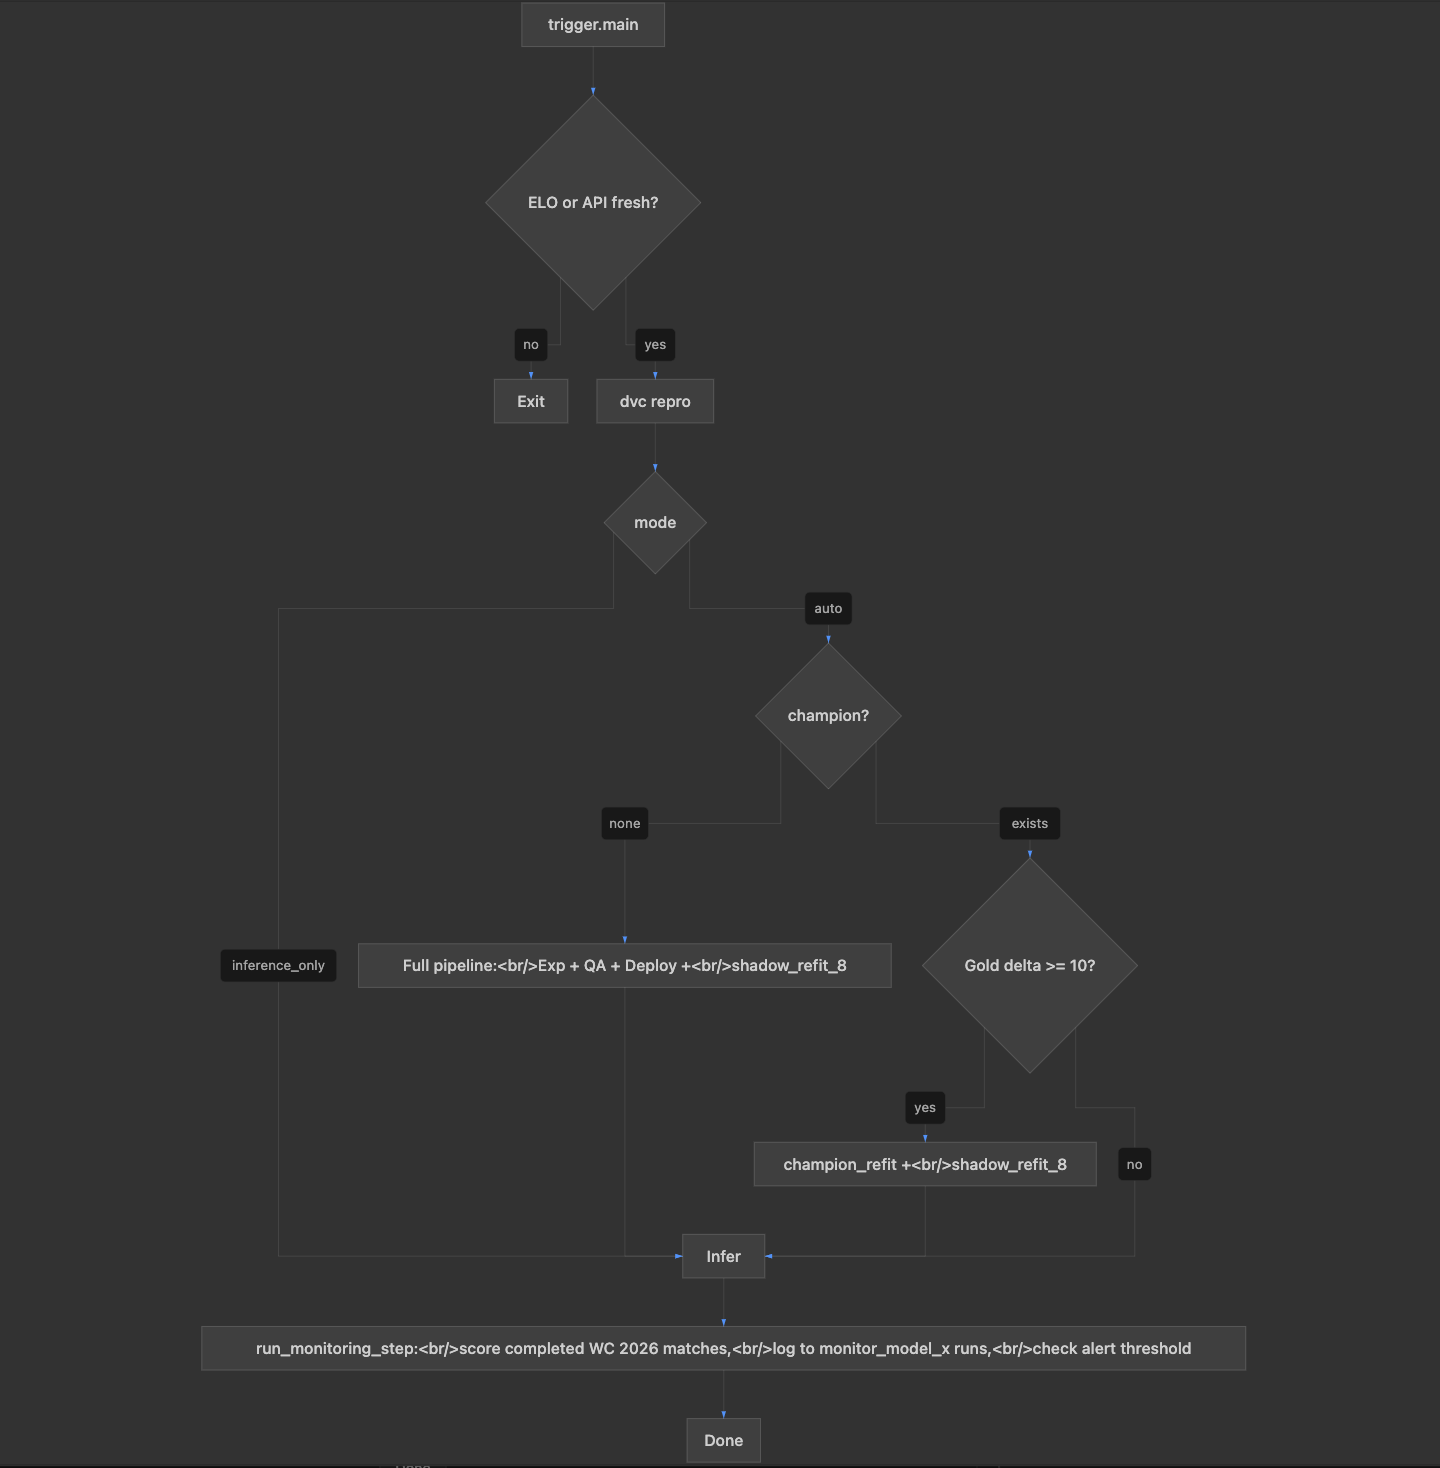
\includegraphics[width=\columnwidth]{../figures/Architecture.png}
  \caption{End-to-end MLOps pipeline architecture.}
  \label{fig:architecture}
\end{figure}

\subsection{Three-Environment Model Lifecycle}

Model development follows a structured three-environment pipeline backed
by three registered MLflow models:

\begin{enumerate}
  \item \textbf{Experimental}: all nine candidate models are trained on the pre-WC 2022
  Gold training split. Hyperparameters are tuned by Optuna using Poisson negative
  log-likelihood (NLL) as the objective. All nine candidates advance
  to QA, sorted by CV NLL.
  \item \textbf{QA}: promoted models are backtested against the 2022 FIFA World Cup.
  The primary KPI is Ranked Probability Score (RPS), with RMSE as secondary metric.
  Each finalist's artifact is serialized and registered as a version
  of \texttt{wc\_staging} in the MLflow model registry; the winner receives
  the \texttt{challenger} alias.
  The best-performing model advances to the deploy phase.
  \item \textbf{Deploy}: the selected model is retrained on the full Gold dataset,
  serialized as an MLflow pyfunc artifact, registered as \texttt{wc\_production}, 
  and used for tournament simulation.
\end{enumerate}

A third registered model, \texttt{wc\_shadow}, holds the eight
non-champion candidates refit on the same full pre-WC~2026 Gold data as
the champion, reusing each candidate's Optuna-tuned hyperparameters.
\texttt{wc\_staging} is the permanent WC~2022 audit trail (training data
ends at the QA cutoff); \texttt{wc\_production} holds only the champion
and feeds the tournament simulation; \texttt{wc\_shadow} feeds the
live-monitoring leaderboard so all nine models can be compared apples-to-
apples on WC~2026 matches without confounding model family with data
recency.

\subsection{Tool Stack}

\begin{table}[h]
  \centering
  \caption{Tool stack}
  \begin{tabular}{ll}
    \toprule
    Purpose & Tool \\
    \midrule
    Data pipeline & Python, pandas, numpy, scipy \\
    Statistical models & statsmodels \\
    Bayesian modeling & PyMC \\
    Hyperparameter tuning & Optuna \\
    ML models & scikit-learn, XGBoost \\
    Deep learning & Keras 3 (JAX backend) \\
    Experiment tracking & MLflow \\
    Data \& artifact versioning & DVC \\
    Code versioning & Git \\
    Testing & pytest \\
    Containerization & Docker \\
    Dashboard & Streamlit, Plotly \\
    Remote collaboration & DagsHub \\
    Cloud deployment & Cloud Run Jobs \\
    \bottomrule
  \end{tabular}
\end{table}

\subsection{Development Timeline}

Figure~\ref{fig:gantt} shows the project timeline.

\begin{figure*}[t]
\centering
\begin{ganttchart}[
    hgrid,
    vgrid,
    x unit=0.18cm,
    y unit title=0.5cm,
    y unit chart=0.6cm,
    title/.style={fill=gray!30},
    title label font=\scriptsize,
    bar label font=\scriptsize,
    group label font=\scriptsize\bfseries,
    bar/.style={fill=blue!40},
    bar incomplete/.style={fill=gray!20},
    milestone/.style={fill=red!70, shape=diamond},
    time slot format=isodate
  ]{2026-03-09}{2026-05-17}
  \gantttitle{March}{23}\gantttitle{April}{30}\gantttitle{May}{17} \\
  \gantttitle{9}{7}\gantttitle{16}{7}\gantttitle{23}{7}\gantttitle{30}{7}%
  \gantttitle{6}{7}\gantttitle{13}{7}\gantttitle{20}{7}\gantttitle{27}{7}%
  \gantttitle{4}{7}\gantttitle{11}{7} \\

  % --- Data Pipeline ---
  \ganttgroup{Data Pipeline}{2026-03-09}{2026-04-30} \\
  \ganttbar{Bronze ingestion}{2026-03-09}{2026-03-15} \\
  \ganttbar{Silver pipeline}{2026-03-16}{2026-03-20} \\
  \ganttbar{Gold v1}{2026-03-23}{2026-03-31} \\
  \ganttbar{Gold v2}{2026-04-27}{2026-04-30} \\

  % --- Modeling ---
  \ganttgroup{Modeling}{2026-03-30}{2026-04-19} \\
  \ganttbar{Experimental env}{2026-03-30}{2026-04-06} \\
  \ganttbar{Pipeline trigger}{2026-03-30}{2026-04-06} \\
  \ganttbar{QA env}{2026-04-01}{2026-04-06} \\
  \ganttbar{Deploy env}{2026-04-03}{2026-04-06} \\
  \ganttbar{MC simulation}{2026-04-13}{2026-04-19} \\

  % --- Monitoring & Deployment ---
  \ganttgroup{Monitoring \& Deployment}{2026-04-27}{2026-05-17} \\
  \ganttbar{Monitoring}{2026-04-27}{2026-05-02} \\
  \ganttbar{Cloud deployment}{2026-05-11}{2026-05-17} \\

  % --- Report (continuous) ---
  \ganttbar{Report write-up}{2026-03-09}{2026-05-17} \\
\end{ganttchart}
\caption{Project timeline (weekly granularity). Data pipeline: Bronze and Silver
complete by 20~March; Gold v1 by 31~March; Gold v2 feature iteration last week of
April. Modeling: all environments and pipeline trigger implemented week of
6~April; Monte Carlo simulation week of 13~April. Monitoring \& Deployment:
monitoring implemented last week of April; cloud deployment (Docker, Cloud Run Jobs,
Cloud Scheduler) week of 11~May~2026. Report write-up is ongoing throughout.}
\label{fig:gantt}
\end{figure*}

% ============================================================
\section{Data Pipeline}
\label{sec:pipeline}

\subsection{Data Sources}

Two external sources provide the input data:

\textbf{API-Football} supplies historical national team fixture results and per-match
statistics (shots, possession, fouls, cards, etc.) for all major international competitions
from 2018 onward. Data is fetched via REST API, stored as date-windowed JSON snapshots in
Bronze, and grouped by league season.

\textbf{Elo ratings} (eloratings.net) provide team strength estimates as tab-separated
historical files, one file per national team. Elo ratings update after each match and offer
a cross-confederation, continuously maintained measure of team quality.

\subsection{Bronze Layer}

Raw data is stored as immutable snapshots. API-Football responses are stored as
\texttt{fixtures.json} and per-match \texttt{\{fixture\_id\}.json} statistics files
in date-windowed subdirectories. Elo TSVs are stored unchanged.
All Bronze artifacts are tracked with DVC; the raw data directory is excluded from Git.

\subsection{Silver Layer}

The Silver pipeline transforms Bronze data into a schema-validated, season-partitioned
Parquet table with one row per finished match. Key transformation steps:

\begin{itemize}
  \item \textbf{Fixture parsing}: only matches with status \texttt{FT}, \texttt{AET},
  or \texttt{PEN} (completed matches) are retained.
  \item \textbf{Statistics join}: per-fixture statistics are joined by \texttt{fixture\_id};
  a \texttt{stats\_tier} column encodes completeness (\texttt{full}, \texttt{core},
  \texttt{partial}, \texttt{none}).
  \item \textbf{Team mapping}: API-Football team IDs are resolved to canonical names
  and ISO country codes via a curated mapping CSV.
  \item \textbf{Filters}: youth squads (e.g.\ \texttt{U21}), B-squads, club teams, and
  non-FIFA entities are removed.
  \item \textbf{Competition tier}: leagues are assigned a tier (1–4) and a binary
  \texttt{is\_knockout} flag using a mapping of competition names and date-based overrides.
  Tier~1 = FIFA World Cup; Tier~2 = continental finals (EURO, Copa América, AFCON, Asian Cup,
  Gold Cup, etc.); Tier~3 = World Cup and continental qualifiers, Nations Leagues;
  Tier~4 = international friendlies (default for unmapped league IDs).
  \item \textbf{Elo join}: pre-match Elo ratings for both teams are joined by date-proximate
  lookup (\texttt{merge\_asof}); the \texttt{is\_neutral} flag is sourced from the Elo
  venue column with a heuristic fallback.
  \item \textbf{Schema validation}: column presence, types, and key constraints are
  verified before writing to Parquet.
\end{itemize}

\subsection{Silver Schema}

The Silver table contains 72 columns per match, organised into six groups
(Table~\ref{tab:silver_schema}). All stat columns are \texttt{Int16} except
possession and pass accuracy (\texttt{Float32}) and pass counts (\texttt{Int32}).
Elo columns are \texttt{Float32}; boolean flags use pandas \texttt{boolean}
(nullable) dtype.

\begin{table}[h]
  \centering
  \caption{Silver layer column groups (72 total)}
  \label{tab:silver_schema}
  \begin{tabular}{lc}
    \toprule
    Column group & Count \\
    \midrule
    Match identity                      & 14 \\
    Teams (API ID, canonical, ISO code, conf.) & 10 \\
    Goals (final, HT, FT, ET, pen.)    & 10 \\
    Elo ratings (pre \& post, both sides) & 4 \\
    Match statistics (16 per side)      & 32 \\
    Quality flags                       & 2  \\
    \midrule
    \textbf{Total}                      & \textbf{72} \\
    \bottomrule
  \end{tabular}
\end{table}

The 16 per-side statistics are: shots on goal, shots off goal, total shots,
blocked shots, shots inside/outside box, fouls, corner kicks, offsides,
possession~\%, yellow cards, red cards, goalkeeper saves, total passes,
accurate passes, and pass accuracy~\%.
Quality flags encode \texttt{has\_statistics} (boolean) and
\texttt{stats\_tier} (\texttt{full} / \texttt{partial} / \texttt{cards\_only}
/ \texttt{none}), derived from which stat subsets are non-null.

\subsection{Gold Layer}

The Gold table contains one row per finished match with all modeling-ready features.
It is produced by \texttt{src.gold.build\_gold} with the following transformations:

\begin{itemize}
  \item \textbf{Rolling form features}: for each team entering a match, we compute
  rolling means of goals for and goals against over the last 10 prior matches (strictly
  before the match date), using all matches regardless of statistics availability.
  Features are computed from the team's perspective regardless of home/away side.
  For teams with fewer than 10 prior matches in the dataset, the window expands to cover
  all available history; only a team's very first match receives a NaN for all rolling
  features.

  \item \textbf{Rolling tactical profiles}: eight per-side rolling mean columns
  capture shot-level and tactical style, computed only from prior matches with
  \texttt{stats\_tier} $\neq$ \texttt{none}.
  Three columns encode shot-level form: \texttt{rolling\_shots} (mean total shots),
  \texttt{rolling\_shot\_accuracy} (shots on goal / total shots), and
  \texttt{rolling\_conversion} (goals / shots on goal).
  Five columns encode tactical style: \texttt{total\_shots} (attacking volume),
  \texttt{shot\_precision} (shots on goal / total shots, NaN-safe for zero denominator),
  \texttt{fouls} (aggressiveness / pressing intensity),
  \texttt{corner\_kicks} (territorial pressure near the opponent goal),
  and \texttt{possession\_pct} (control style).
  Each dimension is intended to capture a distinct tactical axis.
  The original data includes \texttt{shots\_on\_goal}, \texttt{shots\_off\_goal},
  and \texttt{total\_shots} as three separate features, but since these are linearly
  dependent (on-target + off-target $=$ total), taking all of them into account
  individually would triple-weight the shots dimension in Euclidean clustering space
  while adding no orthogonal information. Replacing them with volume
  (\texttt{total\_shots}) and precision (\texttt{shot\_precision}) recovers two
  genuinely independent attacking signals.
  Opponent-suffered statistics (e.g.\ shots conceded) were considered but excluded:
  they confound the team's own tactical style with the quality of opponents faced in
  the rolling window.
  Other detailed columns (e.g.\ \texttt{shots\_insidebox}, \texttt{total\_passes}) are
  excluded due to sparse availability in the \texttt{partial} stats tier
  ($\sim$1.6\% non-null).
  These sixteen columns (eight statistics $\times$ two sides) are used directly as
  continuous model features.

  \item \textbf{Tactical clustering (investigated, not used)}: \texttt{StandardScaler}
  + \texttt{KMeans} clustering on the five rolling tactical columns was evaluated as a
  way to add discrete play-style labels to Gold.  Silhouette and elbow analysis was
  run for $k = 2\ldots10$ across five variants: the full five-column profile, a
  three-column core (\texttt{possession\_pct}, \texttt{total\_shots}, \texttt{fouls}),
  a two-column style proxy (\texttt{possession\_pct}, \texttt{shot\_precision}), and
  PCA reductions to two and three components (Figure~\ref{fig:cluster_k}).
  No variant exceeded a silhouette score of $0.40$; the dominant variance axis across
  all variants was a single volume-and-dominance continuum, not a set of discrete
  tactical archetypes.  This is consistent with rolling averages being computed across
  opponents of varying quality: a team's observed possession or shot count in a
  particular rolling window reflects opponent strength as much as it does the team's
  own style, smoothing out any genuine tactical signal.  Given these results, cluster
  labels were not added to Gold; the ten rolling tactical columns are retained as
  direct continuous features.

  \item \textbf{Elo features}: \texttt{elo\_diff} = \texttt{home\_elo\_pre}
  $-$ \texttt{away\_elo\_pre} represents which side is the favourite in a given
  match based on both teams' match history.  \texttt{elo\_sum} =
  \texttt{home\_elo\_pre} $+$ \texttt{away\_elo\_pre} captures the overall match
  quality (top-vs-top vs bottom-vs-bottom), a non-linear composite that
  tree-based and additive baseline models can split on independently of which
  side is favoured.

  \item \textbf{Squad-cohesion features (time since last national-team match)}:
  for each side, \texttt{home\_days\_since\_last\_match} and
  \texttt{away\_days\_since\_last\_match} record the gap in days to that team's
  previous international match (\texttt{NaN} on first appearance).
  \texttt{rest\_diff} = home $-$ away is the signed difference; \texttt{NaN}
  propagates if either side is missing.  These columns are \emph{not} a
  player-rest signal: at international cadence, players play club
  matches between national-team windows, so individual fatigue is not what
  is measured.  What is measured is \emph{time-as-a-unit}, a proxy for
  squad cohesion, tactical familiarity, set-piece coordination, and roster 
  stability after a recent training window or tournament.  
  The variable name \texttt{rest\_diff} is retained
  from the initial design hypothesis where player rest was the proposed
  mechanism.  Per-team gaps are computed via a team-centric reshape and
  \texttt{groupby('team').shift(1)} on chronologically sorted match
  history (the same pattern as the rolling features); each match's value
  uses only the team's previous match date strictly before the current
  match date.

  \item \textbf{Context features}: \texttt{competition\_tier} (1 = World Cup finals,
  2 = continental finals, 3 = qualifiers/Nations Leagues, 4 = friendlies),
  \texttt{is\_knockout}, \texttt{is\_neutral}, and
  \texttt{is\_cross\_confederation} (nullable boolean: \texttt{True} if the
  two teams' confederations differ; \texttt{NaN} if either confederation is
  missing).  For 2026 WC group-stage matches where a host nation plays at
  home, \texttt{is\_neutral} is overridden to \texttt{False}.

  \item \textbf{Match index}: per-team 1-indexed ordinal match counter used by
  SARIMAX as the integer time axis (not a predictor).

  \item \textbf{Time-awareness guarantee}: every feature uses only information
  from strictly prior matches; the current match's own statistics never appear in
  its feature vector.
\end{itemize}

\begin{figure}[h]
  \centering
  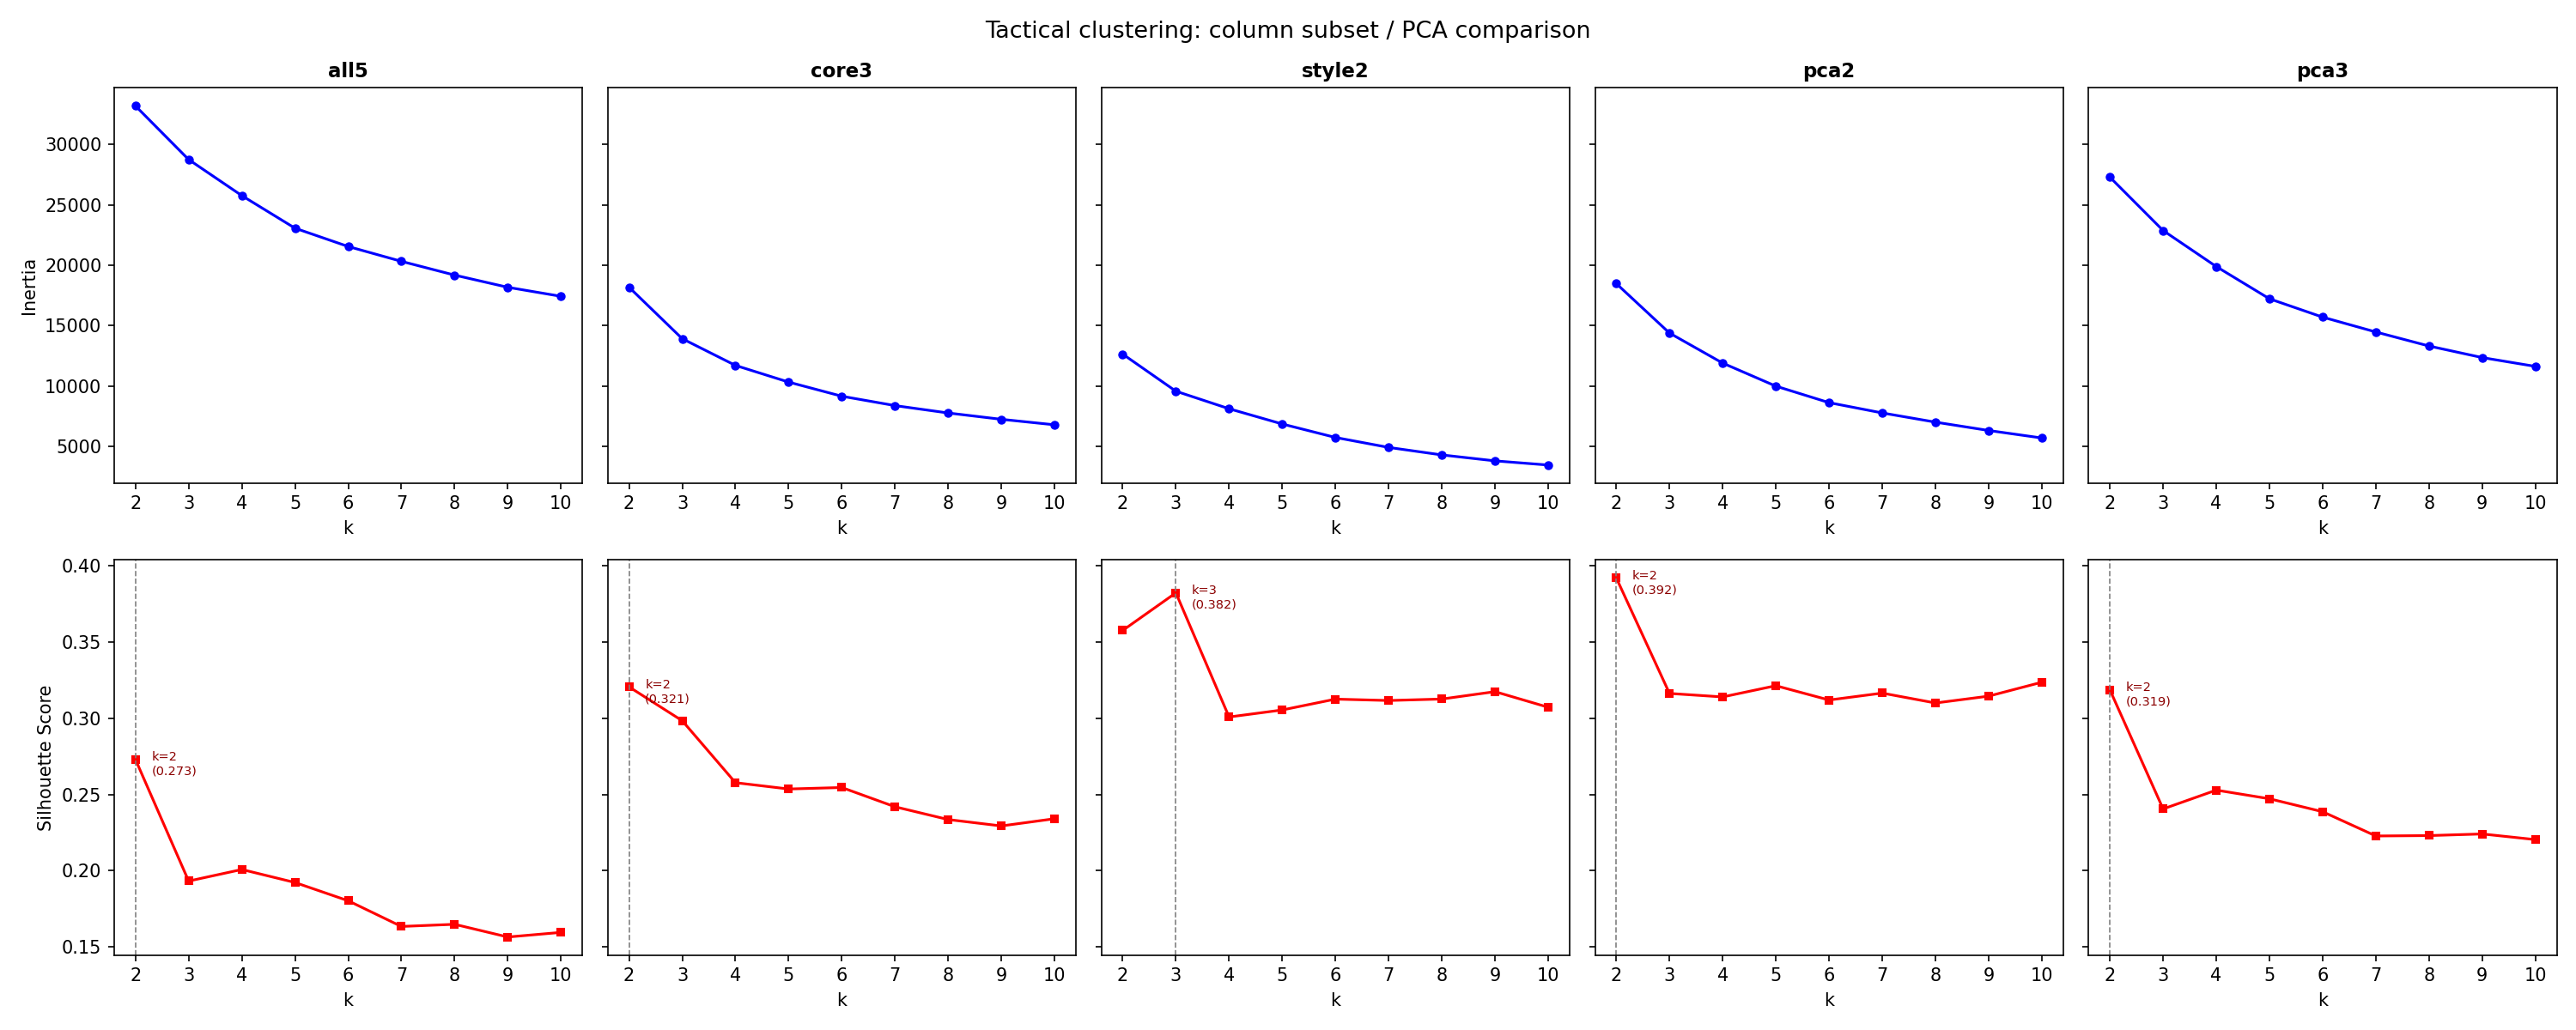
\includegraphics[width=\columnwidth]{../figures/cluster_experiment_v2.png}
  \caption{Elbow (top) and silhouette (bottom) analysis for $k = 2\ldots10$
  across five column-subset and PCA variants of the rolling tactical profile.
  No variant exceeds a silhouette score of $0.40$; all variants peak at $k=2$
  or $k=3$, reflecting a single dominance axis rather than discrete tactical
  archetypes.  Clustering was therefore not included in Gold; the raw rolling
  tactical columns are used as direct continuous features.}
  \label{fig:cluster_k}
\end{figure}

\subsection{Home Advantage at Inference}

The 2026 FIFA World Cup is co-hosted by the United States, Canada, and Mexico, all of
which are participating national teams.  The model learns the home-advantage effect
from the historical \texttt{is\_neutral} flag; no 2026-specific feature is needed.

\textbf{Group stage.}  Each group-stage venue is pre-assigned to a host country.
In the Gold layer, \texttt{override\_neutral\_for\_2026\_hosts()} sets
\texttt{is\_neutral = False} for group-stage rows where a host nation plays at home.
This is deterministic because the venue schedule is known before the tournament.

\textbf{Knockout rounds.}  Venue assignment depends on bracket position, which in turn
depends on group-stage results.  The tournament simulation carries a
\texttt{venue\_country} mapping (venue city $\to$ host country) in
\texttt{wc2026.json}, not Gold features.  When the simulation places a host nation into a
knockout match at a venue in their country, \texttt{is\_neutral} is overridden to
\texttt{False} for that simulated match.  This works identically for deterministic
inference (known bracket) and probabilistic inference (Monte Carlo sampling, where the
override fires only for simulated paths where the host advances to that slot).

\subsection{Ingestion Trigger}

The pipeline trigger (\texttt{src.pipeline.trigger}) checks two data sources
for freshness and executes the pipeline when at least one has new data.
It accepts a \texttt{-{}-mode} argument: \texttt{auto} (retrain if enough new
data, then always infer) or \texttt{inference\_only} (frozen model, predict
and simulate only).

Two freshness checks run on every invocation:

\begin{enumerate}
  \item \textbf{ELO freshness.} All team TSVs are re-downloaded to a temporary
  directory and each file's SHA-256 digest is compared against the last stored
  manifest. At least one digest must have changed.
  \item \textbf{API-Football freshness.} Incremental ingestion runs with a
  48-hour lookback window. The result must contain at least one fixture and
  every fixture in the window must carry a settled status
  (\texttt{FT}, \texttt{AET}, or \texttt{PEN}; no in-progress codes such
  as \texttt{1H}, \texttt{HT}, \texttt{2H}).
\end{enumerate}

The trigger proceeds when \emph{at least one} condition holds (\emph{OR} gate).
An earlier design required both sources to be fresh simultaneously, but this
caused unnecessary pipeline delays when one source lagged the other, which is a
realistic scenario during international windows when Elo ratings update with
a short delay. The Gold layer's date-based join handles alignment naturally:
it only produces rows where both sources have data for the same match,
so running the pipeline with one stale source is safe and never produces
incorrect features.

When only the ELO source is fresh, the trigger re-downloads the ELO TSVs
with overwrite; when only API-Football is fresh, the ELO overwrite is skipped
(API-Football data was already fetched as a side effect of its freshness
check). In both cases, \texttt{dvc repro} rebuilds Silver and Gold from
whatever upstream data is available.

\textbf{Dual-schedule design.}
Two Cloud Scheduler entries invoke the same Cloud Run Job at different
frequencies:
\begin{itemize}
  \item \textbf{Pre-tournament}: daily at 04:30~UTC with
  \texttt{-{}-mode auto}. The time is chosen to ensure that late-evening
  Americas matches have finished and Elo ratings have been updated.
  \item \textbf{Tournament}: every 30~minutes with
  \texttt{-{}-mode inference\_only}, active only during the WC~2026
  date range (June~11 -- July~19). The scheduler entry is created paused
  and manually enabled at tournament start.
\end{itemize}
The Cloud Run Job runs the same Docker image and \texttt{trigger.py} entry
point in both cases; only the \texttt{-{}-mode} argument and schedule differ.
Secrets (API keys, DagsHub credentials) are stored in GCP Secret Manager
and mounted as environment variables at job execution time.

\subsection{Continuous Training and Inference}
\label{sec:ct}

The trigger dispatches one of three paths depending on the mode and
pipeline state (Figure~\ref{fig:ct_architecture}).

\begin{figure}[h]
  \centering
  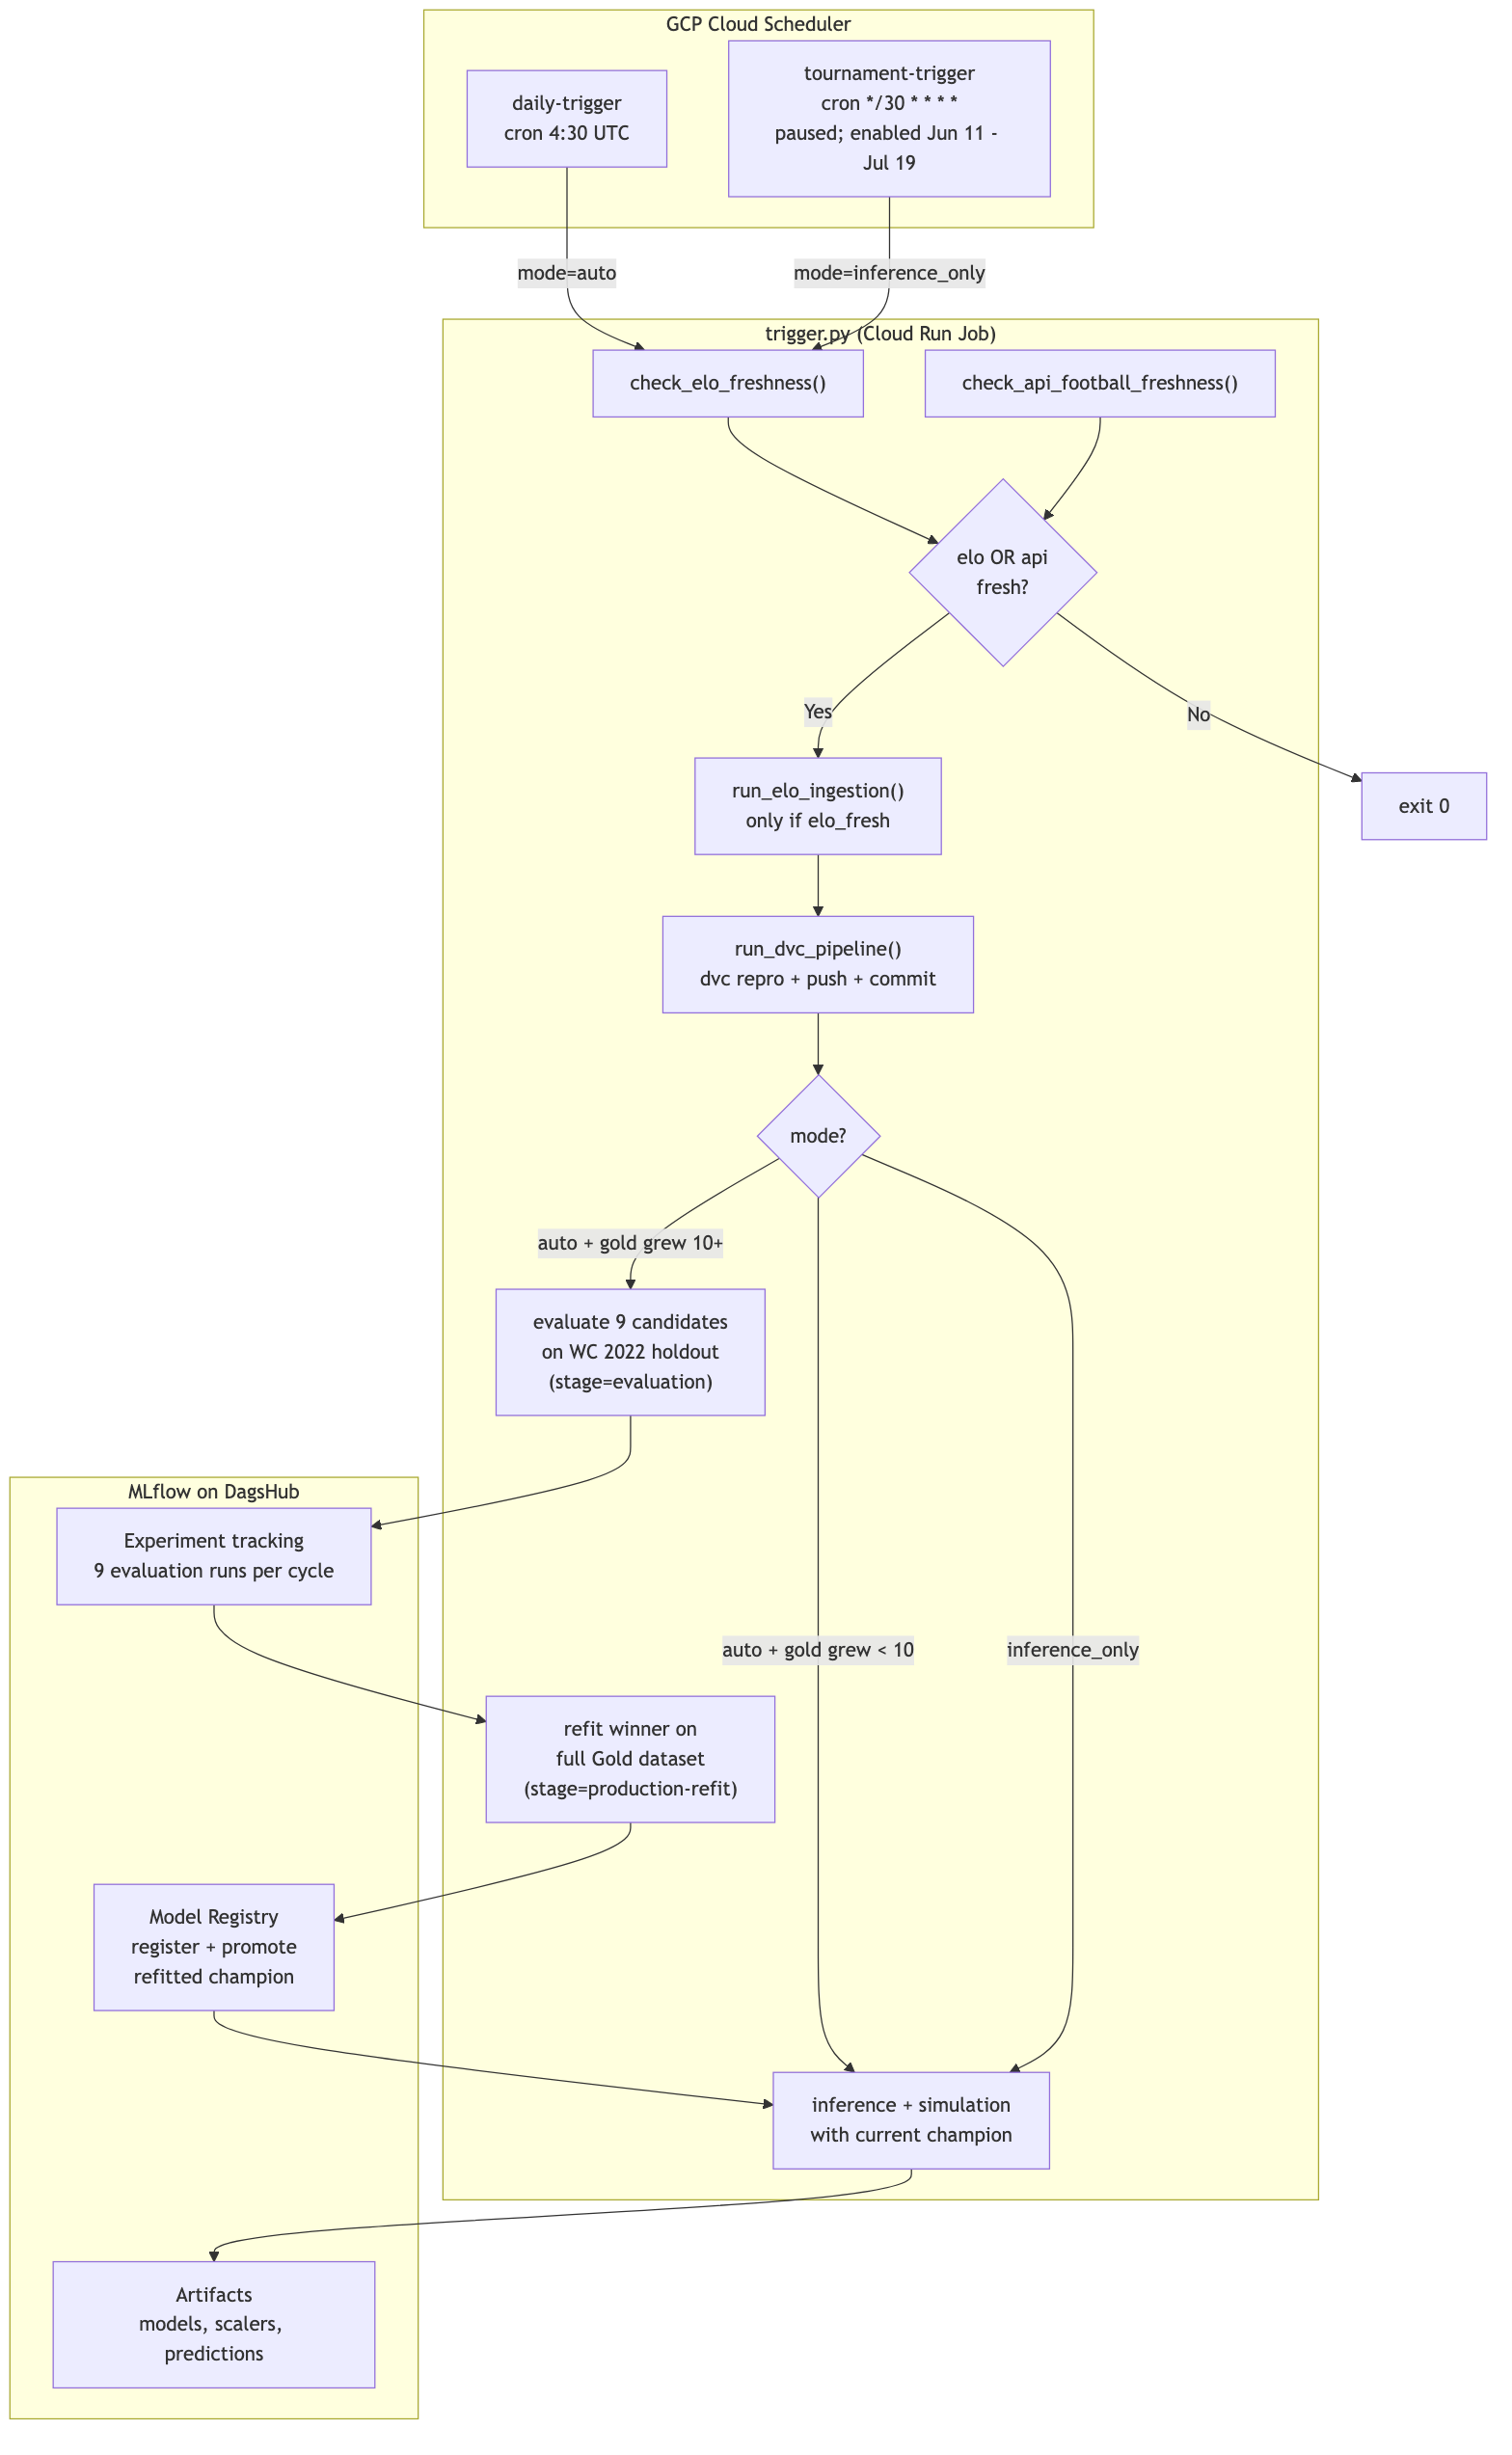
\includegraphics[width=\columnwidth]{../figures/architecture_ct_pipeline.png}
  \caption{Trigger, continuous training, and inference pipeline.
  Pre-tournament: daily trigger refits the champion when Gold grows by
  10+ matches; tournament: 30-minute trigger runs inference only with
  frozen champion.}
  \label{fig:ct_architecture}
\end{figure}

\textbf{Initial model selection (first run).}
When no production champion exists, the trigger executes the full
three-phase pipeline: all nine candidates are tuned via walk-forward
cross-validation (Experimental), evaluated on the 2022 World Cup holdout
(QA), and the best candidate by holdout RPS is promoted via the
\texttt{champion} alias in the MLflow Model Registry.  The champion
architecture and hyperparameters are recorded in the registry.

\textbf{Champion refit (subsequent runs).}
Once a champion exists, the trigger separates \emph{model selection}
(already completed) from \emph{model refresh}.  When Gold has grown by at
least 10 rows since the last training cycle, the trigger loads the
champion's model class and hyperparameters from the MLflow registry, refits
the model on the full Gold dataset available at run time, registers the
new artifact, and promotes it.  The candidate tournament is not re-run:
both the training split and the WC~2022 holdout are fixed by date, so
routine data updates cannot alter model selection.  The QA holdout metrics
from the original selection cycle are forwarded to the refit run for audit
trail continuity.  The full tournament can be re-triggered manually if the
feature set, candidate pool, or evaluation methodology changes.

If Gold grew by fewer than 10 rows, only inference runs.  The retraining
threshold and the last Gold row count are tracked as MLflow run parameters.

\textbf{Shadow refit.}
Whenever a champion refit (or full pipeline) runs, a follow-up
\texttt{run\_shadow\_refit} fits the eight non-champion candidates on the
same full Gold dataset using each candidate's Optuna-tuned
\texttt{best\_params} loaded from the registry. No re-tuning takes place
inside the refit path: model selection is frozen, and re-running
Optuna would both invalidate that contract and add several hours (hardware-dependent)
to every cycle. Each refit is logged as a new MLflow run tagged
\texttt{stage=shadow-refit} and registered as a version of
\texttt{wc\_shadow}; the cold-start case (first install, before
\texttt{wc\_shadow} contains anything) falls back to the
\texttt{wc\_staging} version with the matching \texttt{model\_name} tag,
i.e.\ the QA-phase artifact for that candidate. Shadow refits never feed
the tournament simulation; they exist only to keep the eight
non-champion candidates in sync with the champion's data window so the
monitoring leaderboard (Section~\ref{sec:monitoring_design}) compares
model families on a like-for-like basis.

\textbf{Tournament inference.}
During the tournament, the model is frozen at the parameters established in
the last pre-tournament refit cycle. The 30-minute trigger runs in
\texttt{inference\_only} mode: it first checks for fresh data and, if found,
runs ingestion and \texttt{dvc repro} to rebuild Silver/Gold with updated
rolling averages from any newly completed matches. Already-played WC~2026
results are parsed from the Bronze fixture files (filtered to the current
WC season only, so historical tournaments are excluded) and locked into
the simulation as deterministic constraints. It then loads the
\texttt{champion}-aliased model from the MLflow Model Registry, predicts
expected goal rates for all $\binom{48}{2} = 1{,}128$ possible team
pairings, runs the Monte Carlo tournament simulation with model-derived
rates for every group-stage and knockout matchup, and logs five
inference artifacts to MLflow: per-pairing predicted rates, sampled
scoreline distributions for unplayed group matches, per-team round
advancement probabilities, per-team group-position probabilities, and
per-stage knockout pairing frequencies. The model artifacts are frozen;
only the features are recomputed from the latest data.
No retraining occurs during the tournament.

\textbf{Simulation design.}
The Monte Carlo tournament simulation (\texttt{src.inference.simulation})
draws $n_\mathrm{sims} = 10{,}000$ independent tournament paths.
All $\binom{48}{2}$ team pairings are predicted before simulation, so both
group-stage and knockout matches use model-derived Poisson rates rather than
fallback assumptions.
Group-stage matches are resolved by Poisson scoreline sampling from the
predicted rates. Knockout-round draws after 90~minutes are resolved by sampling extra
time with the same predicted rates scaled by $30/90$ (reflecting the
30-minute extra time period relative to 90-minute regulation). If extra time
also ends in a draw, the outcome is resolved by a 50/50 coin flip, modeling
penalty shootouts as a symmetric random event. Group-stage tiebreakers follow
FIFA rules through goal difference, goals scored, and head-to-head results;
beyond that, fair play points and drawing of lots are approximated by random
tiebreaking. Across all simulations, the engine tracks which team pairs
meet at each knockout stage (R32 through Final). The resulting pairing
frequencies quantify how likely each possible knockout matchup is,
capturing the combinatorial uncertainty introduced by the
best-third-place progressive rule. The $n_\mathrm{sims}$ parameter is
configurable; 10{,}000 is sufficient for stable tournament-level
advancement probabilities without excessive runtime.

% ============================================================
\section{Modeling}
\label{sec:modeling}

\subsection{Modeling Objective}

The primary prediction target is the joint distribution over
$(home\_goals,\; away\_goals)$, not a direct W/D/L classification.
Match outcomes are derived downstream by marginalizing the score distribution:
\begin{equation}
  P(\text{home win}) = \sum_{i > j} P(H=i,\, A=j)
\end{equation}
where $H$ and $A$ are the predicted home and away goal counts.
Monte Carlo tournament simulation samples from the predicted score distributions
to propagate uncertainty through the entire bracket.

\subsection{Candidate Models}

Table~\ref{tab:models} lists the nine candidate models.

\begin{table}[h]
  \centering
  \caption{Candidate models — Experimental environment}
  \label{tab:models}
  \begin{tabular}{clll}
    \toprule
    \# & Model & Family & Library \\
    \midrule
    1 & Poisson GLM         & Statistical   & statsmodels \\
    2 & Negative Binomial GLM & Statistical & statsmodels \\
    3 & Bayesian Poisson    & Bayesian      & PyMC        \\
    4 & SARIMAX (ARIMAX)    & Time-Series   & statsmodels \\
    5 & Ridge Regression    & ML baseline   & scikit-learn \\
    6 & Random Forest       & ML ensemble   & scikit-learn \\
    7 & XGBoost             & ML boosting   & XGBoost      \\
    8 & LSTM                & Deep Learning & Keras        \\
    9 & 1D CNN              & Deep Learning & Keras        \\
    \bottomrule
  \end{tabular}
\end{table}

\textbf{Note on Poisson GLM:} The Poisson GLM implements the bivariate Poisson
distribution of Karlis and Ntzoufras~\cite{karlis2003analysis}. A match is modelled
as three independent Poisson variates, $X_1 \sim \text{Pois}(\lambda_1)$,
$X_2 \sim \text{Pois}(\lambda_2)$, $X_3 \sim \text{Pois}(\lambda_3)$, where
$\text{home\_goals} = X_1 + X_3$ and $\text{away\_goals} = X_2 + X_3$.
The shared component $\lambda_3$ explicitly captures positive score dependence between
sides. Each rate is parameterised as $\exp(\beta^\top x)$ and all three coefficient
vectors are estimated jointly by L-BFGS-B maximum likelihood with an L2 penalty.
This formulation was chosen over the Dixon--Coles~\cite{dixon1997modelling} variant for
two reasons: (i)~the $\lambda_3$ component models positive score dependence across all
scorelines rather than applying a correction only to the four lowest outcomes, providing
a more general dependence structure; and (ii)~the Dixon--Coles time-weighting of older
matches is largely redundant here, because Elo ratings and 10-match rolling form features
already impose implicit recency weighting on the feature side.
A possible extension would be to add explicit likelihood-level time-weighting to the
Karlis--Ntzoufras model to further downweight older matches beyond what these features
capture.

\textbf{Note on Negative Binomial GLM:} The Negative Binomial GLM fits two independent
marginals: one NegBin GLM for home goals and one for away goals, sharing the feature
matrix but no model parameters. This design reflects two practical considerations.
First, the bivariate closure that underpins the Karlis--Ntzoufras construction relies on
Poisson additivity: the sum of independent Poisson variates is again Poisson. Negative
Binomial variates do not share this property under differing dispersion parameters,
making an analogous bivariate extension substantially more complex (requiring either
a shared gamma mixing variable or a copula layer). Second, empirical home/away score
correlation in football is weak (typically $r < 0.10$), so the gain from a full joint
model is modest. The NegBin's primary contribution is relaxing the Poisson
equidispersion assumption; independent marginals retain that benefit without additional
modelling complexity.

\textbf{Note on SARIMAX:} national team matches are irregularly spaced (3--4 days within
international windows, up to 6 months between windows). SARIMAX is applied with an integer
match-index time dimension rather than calendar dates, so the ARIMA component models
serial correlation between consecutive match observations globally. Exogenous variables
are identical to those used by all other models. This simplification is an acknowledged
limitation (Section~\ref{sec:threats}).

\textbf{Note on Bayesian Poisson:} PyMC's NUTS sampler produces full posterior predictive
distributions, which are ideal for propagating uncertainty into Monte Carlo simulation.
Variational inference (ADVI) is used as a faster approximation during experimental runs.

\textbf{Note on Bayesian Bivariate Poisson (excluded):} A Bayesian variant of the
Karlis--Ntzoufras~\cite{karlis2003analysis} bivariate Poisson was implemented and
tested but excluded from the final candidate set. The custom bivariate Poisson
log-PMF---implemented in PyTensor ops via \texttt{pm.CustomDist} with a truncated
$k$-sum---requires PyMC to auto-differentiate through a complex computational graph
(including \texttt{gammaln}, \texttt{logsumexp}, and 2D tensor operations) at every
NUTS leapfrog step. This makes each MCMC step approximately 50$\times$ slower than
the independent-marginals Bayesian Poisson, which uses PyMC's built-in
\texttt{pm.Poisson} with pre-compiled analytical gradients. In a test run with
identical hyperparameter ranges, both models achieved nearly identical CV NLL
($\approx$2.754), indicating that the shared dependence parameter $\lambda_3$ does
not improve predictive accuracy on this dataset. Given the prohibitive computational
cost ($\sim$5--6 hours for 40 Optuna trials vs.\ $\sim$7 minutes for the independent
variant) and no measurable benefit, the model was dropped from the tuning pipeline.
The implementation is retained in the repository for reference.

\subsection{Hypotheses}

\begin{description}
  \item[H1] \textbf{Elo differential is the dominant feature across model families.}
  Elo ratings encode cumulative historical performance and are the most information-dense
  single feature available without squad-level data. Permutation importance is expected to
  rank \texttt{elo\_diff} first across most or all model families, with competition tier
  and rolling form as secondary contributors.

  \item[H2] \textbf{Poisson GLM as a competitive baseline.}
  Football goal counts are well-approximated by Poisson processes~\cite{dixon1997modelling}.
  The Poisson GLM is expected to perform competitively despite its simplicity, providing
  a meaningful floor for more complex models.

  \item[H3] \textbf{XGBoost captures non-linear interactions.}
  Elo differential, competition tier, and rolling form may interact in non-linear ways
  that GLMs cannot capture. XGBoost is expected to outperform linear models by exploiting
  these interactions.

  \item[H4] \textbf{Deep learning models underperform relative to complexity.}
  LSTM and 1D CNN require substantial sequence data to generalize. National team datasets
  are too sparse to fully train deep architectures; both models are expected to underfit
  or overfit relative to simpler alternatives, particularly for teams with short histories.

  \item[H5] \textbf{Bayesian Poisson produces best-calibrated predictions.}
  Calibration matters for tournament simulation. The Bayesian model is expected to yield
  better-calibrated score distributions than point-estimate models, even if its mean
  prediction accuracy is comparable to Poisson GLM.
\end{description}

\subsection{Feature Importance}

Permutation importance is computed for all nine models on the held-out validation set
during the experimental phase. This method is model-agnostic: for each feature, the
validation metric is measured after randomly permuting that feature's values. The
importance score is the resulting metric degradation. Results are logged to MLflow
alongside training metrics and compared across model families in Section~\ref{sec:results}.

% ============================================================
\section{Experimental Setup}
\label{sec:experiments}

\subsection{Training and Validation Split}

The Gold dataset covers international matches from 2018 through 2026.
All matches before the 2022 FIFA World Cup (\texttt{date\_utc < 2022-11-20})
form the training set (3{,}903 rows). Walk-forward expanding-window
cross-validation is applied within this set to tune hyperparameters and
evaluate experimental candidates; the CV folds span the full pre-tournament
period, including 2022 qualification matches. 
The 2022 FIFA World Cup (2022-11-20 to 2022-12-18, 64 matches) is held out
as a strict test set for QA evaluation and is never seen during training or
cross-validation.

\subsection{Evaluation Metric: Ranked Probability Score}

The Ranked Probability Score (RPS) for a single match with $K$ ordered outcome
categories is defined as
\begin{equation}
  \text{RPS} = \frac{1}{K-1} \sum_{k=1}^{K-1}
  \left( \sum_{i=1}^{k} p_i - \sum_{i=1}^{k} o_i \right)^2
\end{equation}
where $p_i$ is the predicted probability and $o_i \in \{0,1\}$ is the observed
indicator for outcome $i$, with outcomes ordered away win, draw, home win ($K=3$).
Lower RPS is better; a perfect prediction scores 0. Unlike accuracy or log-loss, RPS
penalises predictions that assign probability mass to outcomes far from the true result,
making it well-suited for evaluating probabilistic forecasts over ordered categories.
Match-level RPS values are averaged across all matches to yield a single summary score.

\subsection{Tuning Objective: Poisson Negative Log-Likelihood}

RPS is a natural evaluation metric for tournament prediction, since the downstream
application cares about which team advances, i.e.\ outcome-level probabilities, but
it is poorly suited as a \emph{tuning} objective for two reasons.
First, RPS collapses the full score distribution into three ordered W/D/L buckets and
is therefore insensitive to goal-rate accuracy: a model that predicts
$\hat{\lambda}_h = 1.8$ and one that predicts $\hat{\lambda}_h = 2.5$ receive
identical RPS when both imply the same $P(\text{home win})$.
Second, because draw occupies the middle ordinal position, a confident but incorrect
draw prediction never incurs the maximum RPS penalty, creating a subtle incentive
toward draw-hedging in any optimisation loop gated solely by RPS.

The hyperparameter tuning loop therefore uses Poisson negative log-likelihood (NLL):
\begin{equation}
  \text{NLL} = -\frac{1}{N}\sum_{i=1}^{N}
  \bigl[\log P(h_i \mid \hat{\lambda}_{h,i})
       + \log P(a_i \mid \hat{\lambda}_{a,i})\bigr]
\end{equation}
where $h_i, a_i$ are the observed goals and $\hat{\lambda}_{h,i}, \hat{\lambda}_{a,i}$
are the predicted Poisson rates. NLL directly rewards placing probability mass near
the actual scoreline, is agnostic to outcome ordering, and aligns the tuning signal
with the model architecture (all candidates output goal-rate parameters rather than
outcome classes).

RPS remains the gating metric for QA evaluation and champion selection because the
end goal of the pipeline is tournament simulation, where the quantity of operational
interest is the probability that a team wins, draws, or loses each match (and, by
extension, how far it advances). The two metrics thus serve complementary roles:
NLL trains the best possible scoreline predictor; RPS selects the model whose
scoreline predictions translate most faithfully into outcome probabilities.

\subsection{Hyperparameter Tuning}

Hyperparameters are tuned per model using Optuna's Tree-structured Parzen Estimator
(TPE) sampler with 50 trials. Each trial evaluates a candidate configuration via
walk-forward cross-validation on the training set and reports mean CV Poisson NLL as the
objective (with CV RPS logged as a secondary metric). Every trial is logged to MLflow as a nested run under the parent tuning run,
creating a full search audit trail. The best configuration found by Optuna is used for
the final experimental evaluation and all downstream environments.

\subsection{Promotion Gate}
\label{sec:promotion_gate}

All nine candidates advance from the experimental phase to QA, sorted by walk-forward
cross-validation Poisson NLL using their Optuna-tuned hyperparameters.

The initial pipeline design selected only the top four candidates by CV NLL for QA
promotion. The first complete pipeline run revealed a ranking reversal between the
two metrics: the CV NLL ranking (NegBin~$>$~Bayesian~$>$~Poisson~GLM~$>$~XGBoost)
was inverted on the WC~2022 holdout, where XGBoost achieved the lowest RPS and NLL 
despite ranking fourth in CV.  Two observations motivated removing the top-K gate:
\begin{enumerate}
  \item The CV NLL spread across all nine models was narrow
  (2.753--3.010), making the cutoff between rank~4 and rank~5 fragile: a
  difference of $<0.005$ in CV NLL separated promoted from excluded candidates.
  \item QA evaluation of all nine models adds approximately two minutes of
  wall-clock time (the QA phase retrains and evaluates each model on 89
  holdout matches), negligible compared to the multi-hour
  experimental phase.
\end{enumerate}
Advancing all nine models to QA ensures that no candidate is excluded based
on a metric that proved to be a poor predictor of holdout performance on this
dataset.  The champion/challenger gate in the deploy phase
(Section~\ref{sec:experiments}) remains the sole quality gate for production
promotion.

\subsection{QA Evaluation — 2022 World Cup Backtest}

Promoted models are evaluated on 64 matches from the 2022 FIFA World Cup (Qatar).
Reported KPIs:
\begin{itemize}
  \item \textbf{Ranked Probability Score (RPS)}: average over all matches; lower is better.
  Used as the champion/challenger gate metric.
  \item \textbf{Holdout NLL}: Poisson negative log-likelihood on the holdout set, identical
  to the tuning objective but computed on the WC~2022 matches. Reported alongside RPS to
  preserve scoreline-level signal that RPS collapses into three W/D/L buckets. Not used
  for gating; informational only.
  \item \textbf{RMSE (home goals)}: root mean squared error between the
  predicted home-goal rate $\hat{\lambda}_h$ and the actual home goals.
  \item \textbf{RMSE (away goals)}: same for the away-goal rate
  $\hat{\lambda}_a$.
\end{itemize}

\subsection{Champion Selection and Production Refit}
All QA finalists are serialized and registered as versions of
\texttt{wc\_staging} in the MLflow model registry during the QA phase
(Section~\ref{sec:experiments}).  These artifacts are trained on the
pre-WC~2022 split and serve as the permanent audit trail for the
WC~2022 holdout numbers reported in Section~\ref{sec:results}; they are
\emph{not} used for inference, and they are explicitly distinct from
\texttt{wc\_shadow}, the registered model that holds the eight
non-champion candidates refit on the full pre-WC~2026 Gold dataset for
live-monitoring purposes (Section~\ref{sec:monitoring_design}).

The QA candidate with the lowest holdout RPS is designated the challenger
and receives the \texttt{challenger} alias on \texttt{wc\_staging}.
If no current champion exists, the challenger is promoted unconditionally.
Otherwise, promotion requires the challenger's holdout RPS to strictly
improve on the current champion's recorded RPS; if it does not,
\texttt{ChallengeFailed} is raised and the existing champion is retained.
On successful promotion, the champion model is refit on \emph{all} available
Gold data (\texttt{X\_full}, covering 2018 through the latest ingested match)
using the hyperparameters selected during the experimental phase.
This production-refit artifact is distinct from the QA version:
it is serialized as a new MLflow pyfunc artifact, registered as a version of
\texttt{wc\_production}, and promoted via the \texttt{champion} alias.
The \texttt{wc\_staging} QA versions are retained for audit and comparison.
The associated MLflow run records the QA holdout metrics
(\texttt{qa\_holdout\_rps}, \texttt{qa\_holdout\_rmse\_home},
\texttt{qa\_holdout\_rmse\_away}) together with the full Gold row count and
the QA run ID for traceability.

\textbf{Subsequent automated refits.}
After the initial model selection, subsequent trigger cycles that exceed the
retraining threshold bypass the candidate tournament entirely.  The trigger
loads the champion's model class and hyperparameters from the MLflow
registry and refits the model on the latest full Gold dataset.  The original
QA holdout metrics are forwarded unchanged to the new MLflow run, preserving
audit continuity without re-evaluating on the fixed WC~2022 holdout (which
would produce identical results, since neither the training split nor the
holdout changes with new data).  This separation of model selection from
model refresh avoids a redundant multi-hour candidate tournament on
every data update while maintaining a complete versioned history of
production artifacts in MLflow.

% ============================================================
\section{Results}
\label{sec:results}

\subsection{Experimental Phase — Cross-Validation Results}

Table~\ref{tab:cv_results} reports the walk-forward cross-validation Poisson NLL
for all nine candidate models, sorted from best to worst.  The top three models
by CV NLL are statistical models (NegBin GLM, Bayesian Poisson, Poisson GLM),
followed by the tree-based models (XGBoost, Random Forest).  Deep learning
models (LSTM, CNN), Ridge regression, and SARIMAX occupy the lower ranks.

\begin{table}[h]
  \centering
  \caption{Experimental phase --- Walk-forward CV Poisson NLL (lower is better).
  All nine candidates advance to QA.}
  \label{tab:cv_results}
  \begin{tabular}{clc}
    \toprule
    Rank & Model & CV NLL \\
    \midrule
    1 & Negative Binomial GLM & 2.7576 \\
    2 & Bayesian Poisson      & 2.7587 \\
    3 & Poisson GLM           & 2.7631 \\
    4 & XGBoost               & 2.7665 \\
    5 & Random Forest         & 2.7684 \\
    6 & LSTM                  & 2.8207 \\
    7 & Ridge                 & 2.8471 \\
    8 & SARIMAX               & 3.0161 \\
    9 & 1D CNN                & 3.0393 \\
    \bottomrule
  \end{tabular}
\end{table}

The spread between the best and worst model is 0.282 in NLL; among the top
five models, the spread is only 0.011.  This narrow range foreshadows the
tight QA results and motivates advancing all nine candidates to the holdout
evaluation (Section~\ref{sec:promotion_gate}).

\subsection{QA Phase — 2022 World Cup Holdout}

Table~\ref{tab:qa_results} reports holdout metrics for all nine candidates
evaluated on the 64 matches of the 2022 FIFA World Cup.

\begin{table}[h]
  \centering
  \caption{QA phase --- WC~2022 holdout metrics (sorted by RPS, lower is better).
  The champion/challenger gate uses holdout RPS as the primary KPI.}
  \label{tab:qa_results}
  \begin{tabular}{clcccc}
    \toprule
    Rank & Model & \footnotesize{Holdout RPS} & \footnotesize{Holdout NLL}
         & \footnotesize{RMSE$_h$} & \footnotesize{RMSE$_a$} \\
    \midrule
    1 & XGBoost          & \textbf{0.2109} & 2.916 & 1.388 & 1.095 \\
    2 & Random Forest    & 0.2121 & 2.923 & 1.380 & 1.107 \\
    3 & Ridge            & 0.2141 & 2.964 & 1.428 & 1.080 \\
    4 & Poisson GLM      & 0.2159 & 2.953 & 1.423 & 1.141 \\
    5 & Bayesian Poisson & 0.2166 & 2.964 & 1.436 & 1.144 \\
    6 & NegBin GLM       & 0.2170 & 2.967 & 1.436 & 1.150 \\
    7 & SARIMAX          & 0.2183 & 3.262 & 1.430 & 1.106 \\
    8 & LSTM             & 0.2207 & 2.964 & 1.443 & 1.103 \\
    9 & 1D CNN           & 0.2248 & 3.065 & 1.526 & 1.086 \\
    \bottomrule
  \end{tabular}
\end{table}

XGBoost wins with a holdout RPS of 0.2109, despite ranking only fourth by
CV NLL (2.7665).  The CV NLL winner (NegBin GLM, 2.7576) drops to sixth
in holdout RPS (0.2170).  This ranking reversal is discussed further in
Section~\ref{sec:discussion}.  Excluding 1D CNN, the remaining eight
models fall within a 0.0098 RPS band (0.2109--0.2207).  LSTM, which had
ranked second in the v1 feature configuration with RPS 0.2133, dropped to
rank 8 (RPS 0.2207) after the Gold v2 feature expansion; this regression
is examined in Section~\ref{sec:gold_v2}.

XGBoost was promoted to the production champion alias.  A prior champion
existed (the v1 XGBoost configuration, holdout RPS 0.2118), so promotion
was conditional on strict improvement: v2 XGBoost beat v1 by $\Delta\,$RPS
$= -0.0009$, satisfying the champion/challenger gate
(Section~\ref{sec:promotion_gate}) and triggering automated registration as
\texttt{wc\_production} version~4.  The v1 $\to$ v2 transition is the
subject of Section~\ref{sec:gold_v2}.

\subsection{Feature Importance}

Table~\ref{tab:importance} summarises the top-3 features by permutation
importance (NLL degradation) for each model.  The \texttt{elo\_diff}
feature dominates across all nine models, with importance scores one to
two orders of magnitude above any other feature.  Permutation importance
is computed on experimental-phase CV folds over the full 2018--2026
training window, i.e.\ on a distribution where the large majority of
matches are non-neutral (qualifiers, friendlies, Nations League);
home/away labels are therefore meaningful, in contrast to the
near-fully-neutral 2022 World Cup holdout used in QA.

\begin{table*}[t]
  \centering
  \caption{Top-3 features by permutation importance (RPS degradation).
  \texttt{elo\_diff} ranks first in all nine models.}
  \label{tab:importance}
  \begin{tabular}{lccc}
    \toprule
    Model & \#1 & \#2 & \#3 \\
    \midrule
    Random Forest & \texttt{elo\_diff} \scriptsize{+.121}
      & \texttt{elo\_sum} \scriptsize{+.002}
      & \texttt{roll\_goals\_ag$_h$} \scriptsize{+.002} \\
    SARIMAX & \texttt{elo\_diff} \scriptsize{+.110}
      & \texttt{roll\_goals\_ag$_h$} \scriptsize{+.002}
      & \texttt{elo\_sum} \scriptsize{+.000} \\
    NegBin GLM & \texttt{elo\_diff} \scriptsize{+.104}
      & \texttt{roll\_goals\_ag$_h$} \scriptsize{+.001}
      & \texttt{comp\_tier} \scriptsize{+.001} \\
    Bayesian Poisson & \texttt{elo\_diff} \scriptsize{+.103}
      & \texttt{rest\_diff} \scriptsize{+.001}
      & \texttt{roll\_goals\_ag$_h$} \scriptsize{+.001} \\
    Poisson GLM & \texttt{elo\_diff} \scriptsize{+.102}
      & \texttt{roll\_goals\_ag$_h$} \scriptsize{+.001}
      & \texttt{comp\_tier} \scriptsize{+.001} \\
    XGBoost & \texttt{elo\_diff} \scriptsize{+.098}
      & \texttt{roll\_tac\_poss$_a$} \scriptsize{+.002}
      & \texttt{roll\_goals\_ag$_h$} \scriptsize{+.002} \\
    LSTM & \texttt{elo\_diff} \scriptsize{+.095}
      & \texttt{is\_neutral} \scriptsize{+.005}
      & \texttt{comp\_tier} \scriptsize{+.002} \\
    Ridge & \texttt{elo\_diff} \scriptsize{+.062}
      & \texttt{roll\_goals\_ag$_h$} \scriptsize{+.004}
      & \texttt{roll\_goals\_ag$_a$} \scriptsize{+.002} \\
    1D CNN & \texttt{elo\_diff} \scriptsize{+.055}
      & \texttt{is\_neutral} \scriptsize{+.005}
      & \texttt{comp\_tier} \scriptsize{+.004} \\
    \bottomrule
  \end{tabular}
\end{table*}

Three patterns stand out beyond the \texttt{elo\_diff} dominance.
First, XGBoost is the only candidate whose top three contains a tactical
rolling feature (\texttt{away\_team\_rolling\_tac\_possession\_pct}).
This is partly structural, since XGBoost is the only model that receives
the full 29-feature set, so the other eight were never offered the
tactical columns to rank, but the feature is still chosen over the
nine other tactical columns that XGBoost did have access to, and
specifically in its \emph{away}-side variant.  The permutation gain is
small ($+0.002$ $\Delta$ NLL) and should be read as suggestive rather
than conclusive; possible interpretations are developed in
Section~\ref{sec:discussion}.
Second, two of the five Gold-v2 features surface in top-3 importance:
\texttt{elo\_sum} for Random Forest (a non-linear ``match quality'' split
that the tree can branch on independently of which side is favoured) and
\texttt{rest\_diff} for Bayesian Poisson (the only family whose
prior-driven sampler exploits the squad-cohesion signal).  The other
three Gold-v2 features (\texttt{home\_days\_since\_last\_match},
\texttt{away\_days\_since\_last\_match}, and
\texttt{is\_cross\_confederation}) do not appear in any model's top
three; the per-feature interpretation is developed in
Section~\ref{sec:gold_v2}.
Third, the deep learning models (LSTM, CNN) assign notably higher
importance to \texttt{is\_neutral} than any other model family, suggesting
they rely more heavily on the venue signal to compensate for their weaker
exploitation of the Elo differential.

% ============================================================
\section{Discussion}
\label{sec:discussion}

\subsection{Hypothesis Evaluation}

\textbf{H1: Elo features are the dominant feature family --- confirmed.}
\texttt{elo\_diff} ranks first in permutation importance across all nine
model families (Table~\ref{tab:importance}), with importance scores ranging
from $+0.055$ (CNN) to $+0.121$ (Random Forest), one to two orders of
magnitude above any other feature.  \texttt{elo\_sum}, the second Elo
feature added in the Gold v2 iteration, surfaces in the top three for
Random Forest and SARIMAX (Section~\ref{sec:gold_v2}), giving Elo
information two distinct top-rank entries in those families.  The
remaining secondary features (\texttt{rolling\_goals\_against},
\texttt{competition\_tier}) contribute importance on the order of
$10^{-3}$, confirming that Elo encodes the vast majority of accessible
predictive signal in this dataset.

\textbf{H2: Poisson GLM as competitive baseline --- confirmed.}
Poisson GLM ranks third in CV NLL (2.7631) and fourth in holdout RPS
(0.2159), within 0.005 of the champion.  It outperforms Bayesian Poisson,
NegBin GLM, SARIMAX, LSTM, and CNN on holdout RPS, demonstrating that
the classical Poisson assumption provides a strong baseline that more
complex models struggle to substantially improve upon.

\textbf{H3: XGBoost captures non-linear interactions --- partially
confirmed.}
XGBoost wins the holdout evaluation (RPS 0.2109) despite ranking fourth in
CV NLL, suggesting it captures interactions that improve out-of-sample
generalisation.  This v2 XGBoost configuration was auto-promoted over the
prior v1 champion (Section~\ref{sec:gold_v2}).  It is also the only model
whose top-three importance contains a tactical feature
(\texttt{away\_team\_rolling\_tac\_possession\_pct}), enabled by its access
to the full 29-feature set.  One plausible reading is that rolling
possession is a \emph{dominance} marker that partially overlaps with
\texttt{elo\_diff} --- consistent with the volume-and-dominance continuum
observed in the clustering experiment (Figure~\ref{fig:cluster_k}) --- but
encodes a residual playstyle axis that Elo, which scores results rather
than the manner in which they are obtained, does not fully absorb.  The
fact that it is specifically the \emph{away}-side variant that surfaces is
suggestive: home possession is confounded with the home-advantage effect,
whereas sustained away possession has to be imposed against both the
opponent and the venue, making it a cleaner proxy for proactive style
that XGBoost can then combine non-linearly with \texttt{elo\_diff}.
Importantly, the permutation importance is only $+0.002$ $\Delta$ NLL, so
this interpretation is offered as a hypothesis rather than a confirmed
mechanism.

\textbf{H4: Deep learning underperforms relative to complexity ---
confirmed (and sharper after v2).}
CNN ranks last (RPS 0.2248), confirming the expected data-sparsity penalty
for deep architectures.  LSTM, which had ranked second under the v1
configuration (RPS 0.2133), regressed to rank eight under v2 (RPS 0.2207
--- $\Delta$ RPS $+0.0074$).  Adding five features to a national-team
corpus that already strains sequence-model capacity sharpens the original
hypothesis: the deeper the input dimensionality relative to the available
sequence length, the more pronounced the data-sparsity penalty becomes.
The v1 LSTM result was the most surprising number in the original study
(rank 2 from a model family expected to underfit); the v2 result places
LSTM where the hypothesis predicted it should be, and the regression
itself becomes diagnostic evidence for H4 rather than a counterexample
(Section~\ref{sec:gold_v2}).

\textbf{H5: Bayesian Poisson produces best-calibrated predictions --- not
confirmed.}
Bayesian Poisson ranks fifth in holdout RPS (0.2166), behind XGBoost,
Random Forest, Ridge, and Poisson GLM.  Its holdout NLL (2.9642) is also
higher than XGBoost's (2.9155) and Poisson GLM's (2.9532).  The posterior
predictive distributions produced by ADVI do not translate into superior
W/D/L calibration on this holdout set.  A possible explanation is that
ADVI provides a mean-field Gaussian approximation to the true posterior,
which may underestimate predictive variance and thus lose the calibration
advantage that full MCMC sampling would provide.  Bayesian Poisson is,
however, the one model that exploits the squad-cohesion signal added in
the Gold v2 iteration (\texttt{rest\_diff} ranks second in its
importance). This is consistent with prior-driven samplers being more receptive
to weak-but-real signals than maximum-likelihood baselines
(Section~\ref{sec:gold_v2}).

\textbf{SARIMAX.}
SARIMAX ranks seventh in holdout RPS (0.2183) and last in holdout NLL
(3.262), substantially higher than all other models.  The integer
match-index time axis, which treats multi-month gaps identically to
within-window spacing, likely limits its ability to capture meaningful
temporal structure (Section~\ref{sec:threats}).

\subsection{Feature Iteration: Gold v2}
\label{sec:gold_v2}

\textbf{Motivation.}
After the initial nine-model evaluation produced a stable champion, we used
the platform to test whether five additional engineered features improve
out-of-sample performance.  The features were chosen to address gaps in the
original Core feature set: cross-team strength composition (\texttt{elo\_sum}),
squad-cohesion proxies (\texttt{home\_days\_since\_last\_match},
\texttt{away\_days\_since\_last\_match}, \texttt{rest\_diff}), and a
confederation-mismatch indicator (\texttt{is\_cross\_confederation}).
Methodology was held constant: same nine architectures, same train/CV/holdout
splits, same Optuna budgets --- only the feature columns changed.
\texttt{CORE\_FEATURE\_COLUMNS} grew from 8 to 13; \texttt{FULL\_FEATURE\_COLUMNS}
(XGBoost only) from 24 to 29.

\textbf{Outcome.}
The full pipeline re-ran end-to-end.  The auto-promotion gate
(Section~\ref{sec:promotion_gate}) accepted v2 XGBoost over v1 XGBoost:
holdout RPS $0.2109$ vs $0.2118$ ($\Delta\,$RPS $= -0.0009$), a narrow but
real improvement that triggered registration as \texttt{wc\_production}
version~4.  The CV NLL phase regressed slightly across the board
($\Delta \approx +0.005$ to $+0.06$), consistent with feature additions
raising variance in early walk-forward folds where per-team histories are
shortest; the WC~2022 holdout, where features have stabilised across the
full 2018--2022 training window, is the gating signal.

\begin{table}[h]
  \centering
  \caption{Per-model v1 $\to$ v2 holdout RPS deltas. Tree models improved;
  GLMs and Bayesian Poisson regressed slightly; LSTM regressed measurably.
  Auto-promotion fired for the v2 XGBoost configuration.}
  \label{tab:gold_v2_deltas}
  \begin{tabular}{lccc}
    \toprule
    Model & v1 RPS & v2 RPS & $\Delta$ \\
    \midrule
    \textbf{XGBoost}$^{\ast}$ & 0.2118 & \textbf{0.2109} & $-0.0009$ \\
    Random Forest    & 0.2148 & 0.2121 & $-0.0027$ \\
    1D CNN           & 0.2296 & 0.2248 & $-0.0048$ \\
    Ridge            & 0.2136 & 0.2141 & $+0.0004$ \\
    SARIMAX          & 0.2178 & 0.2183 & $+0.0005$ \\
    Poisson GLM      & 0.2148 & 0.2159 & $+0.0011$ \\
    NegBin GLM       & 0.2155 & 0.2170 & $+0.0015$ \\
    Bayesian Poisson & 0.2149 & 0.2166 & $+0.0017$ \\
    LSTM             & 0.2133 & 0.2207 & $+0.0074$ \\
    \bottomrule
  \end{tabular}
  \\[2pt]
  \footnotesize{$^{\ast}$ Auto-promoted to \texttt{wc\_production} version~4.}
\end{table}

\textbf{Tree models benefit.}
Random Forest improved most ($\Delta\,$RPS $= -0.0027$): \texttt{elo\_sum}
gives it a non-linear ``match quality'' split that linear models cannot
exploit, and the v2 importance places \texttt{elo\_sum} second behind
\texttt{elo\_diff} for this model.  XGBoost improved more modestly
($-0.0009$) because it can already reconstruct any monotonic combination
of \texttt{home\_elo\_pre} and \texttt{away\_elo\_pre} natively via tree
splits, so \texttt{elo\_sum} is partially redundant for the gradient
booster but still provides a marginal benefit by reducing the depth at
which the same information becomes available.

\textbf{GLMs and Bayesian regress slightly.}
Four of the five additive baseline models (Poisson GLM, NegBin GLM,
Bayesian Poisson, SARIMAX) regressed by $+0.0005$ to $+0.0017$ RPS;
Ridge stayed approximately flat ($+0.0004$).  Adding five features
without strong regularisation introduces noise that low-capacity
additive models cannot suppress: each new feature receives an estimated
coefficient that absorbs sample variance, and three of the five new
features carry near-zero true signal for these architectures.  This is
the textbook bias--variance tradeoff for low-capacity models on a
fixed-size training set.

\textbf{LSTM regresses measurably.}
LSTM degraded by $+0.0074$ RPS, the largest regression in the comparison.
A sequence model trained on a sparse national-team corpus is already
operating near its capacity ceiling; adding 5 features to a 13-feature
input deepens the data-sparsity penalty disproportionately, since
recurrent weight matrices scale with input dimensionality.  As discussed
in the H4 paragraph above, this regression is itself diagnostic: it
confirms the original hypothesis on a controlled second observation and
relocates LSTM in the ranking to where the architectural argument
predicted it should be.

\textbf{Feature-level findings.}
\texttt{elo\_sum} is the most consistently useful new feature, appearing
in top-5 importance for four of the nine models (Random Forest \#2,
SARIMAX \#3, NegBin GLM \#4, Poisson GLM \#5).  It captures the
``high-quality matchup'' axis that is non-linear in
\texttt{home\_elo\_pre} $\!+\!$ \texttt{away\_elo\_pre} and orthogonal to
\texttt{elo\_diff}.  The squad-cohesion features (\texttt{rest\_diff},
\texttt{away\_days\_since\_last\_match}) only register for Bayesian
Poisson (top-5 entries at \#2 and \#4); the other eight models suppress
these as noise.  The interpretation is that prior-driven samplers can
absorb weak-but-real signals where maximum-likelihood baselines cannot,
and at international cadence the cohesion gap between teams is mostly
noise across most matchups but carries real information when the composition of one side
changed significantly since the most recent training and match window.
\texttt{is\_cross\_confederation} is invisible in all model importances:
it is heavily confounded with \texttt{competition\_tier} (most
cross-confederation matches are friendlies), so the model already had
access to the same signal under a different name.  It is a reasonable
removal candidate in a future iteration, retained here for schema
stability.

\textbf{Methodology takeaway.}
The auto-promotion machinery did its job: it accepted a marginal-but-real
improvement and would have rejected one that fell below the prior
champion's holdout bar.  This is the iteration loop the MLOps design is
built for; v2 demonstrates the loop closing on real data without manual
intervention.  The mixed per-model results (winners, losers, and one
invisible feature) also illustrate that the gate is doing meaningful
selection rather than rubber-stamping.  Both v1 and v2 artifacts remain
in the MLflow registry as versioned production candidates, so the
iteration is auditable end-to-end.

\subsection{CV--Holdout Ranking Reversal}

The most notable structural result, persisting across both v1 and v2
configurations, is the ranking reversal between the experimental and QA
phases.  The top-three CV NLL models (NegBin GLM, Bayesian Poisson,
Poisson GLM) all drop to the lower half of the holdout RPS ranking,
while XGBoost rises from fourth to first.  This divergence has two
plausible explanations:

\begin{enumerate}
  \item \textbf{Metric mismatch.}  CV NLL operates in goal-count space
  and rewards models that place probability mass near the observed
  scoreline.  Holdout RPS collapses the score distribution into three
  W/D/L buckets.  A model that is well-calibrated at the scoreline level
  may not be optimal at the outcome-probability level, and vice versa.
  \item \textbf{Distribution shift.}  The WC~2022 holdout is a
  tournament-only sample of 89 matches with higher average competitive
  stakes, more neutral venues, and stronger teams than the training set
  average.  Models that overfit to the distributional characteristics of
  the training period (which includes many tier-3 and tier-4 matches) may
  generalise less well to a tournament environment.  XGBoost's ability to
  learn non-linear decision boundaries may make it more robust to this
  shift.
\end{enumerate}

This reversal was the empirical motivation for removing the original
top-four promotion gate (Section~\ref{sec:promotion_gate}): had the gate
remained, Random Forest (rank~5 in CV NLL but rank~2 in holdout RPS) and
Ridge (rank~7 in CV NLL but rank~3 in holdout RPS) would have been
excluded from QA based on a CV metric that proved misleading.

\subsection{Narrow Result Spread}

Excluding CNN, the remaining eight models cluster within a 0.0098 holdout
RPS band (0.2109--0.2207).  Three structural factors explain this:

\begin{enumerate}
  \item \textbf{Shared feature ceiling.} All core-feature models consume the
  same 13 features, with Elo differential accounting for the majority of
  predictive signal (Table~\ref{tab:importance}).  Model architecture
  differences can only exploit the residual variance beyond what Elo already
  captures.

  \item \textbf{Low-signal football domain.} National team football is
  inherently noisy: small squads, irregular calendars, and frequent upsets
  limit the achievable prediction accuracy for any model family.

  \item \textbf{RPS collapses score distributions.} RPS evaluates three
  cumulative W/D/L probabilities. Two models that produce meaningfully
  different goal-rate distributions can nonetheless yield near-identical RPS
  when their W/D/L marginals agree. Holdout NLL is reported alongside RPS
  precisely because it preserves scoreline-level differences that RPS
  discards.
\end{enumerate}

The practical implication is that champion selection in this domain is
sensitive to the holdout sample: a different 89-match tournament could
plausibly produce a different ranking among the top eight models.  This
reinforces the value of advancing all candidates to QA and treating the
champion/challenger gate as the sole decisive quality threshold.

% ============================================================
\section{Threats to Validity}
\label{sec:threats}

\subsection{Data Quality}

\textbf{Sparse statistics coverage.}
Approximately 51\% of matches contain any per-match statistics; coverage is substantially
lower for CAF, AFC, and OFC confederation matches. Models that include statistics-based
features operate on a reduced effective training set for non-European and non-South-American
teams, which may reduce reliability when predicting their matches against the UEFA and CONMEBOL teams that are disproportionately represented in later World Cup stages.

\textbf{Dual-source identity mismatch.}
API-Football and Elo use different team name conventions and country codes. Resolution
relies on a manually curated mapping file. Any future team renaming or code change
requires a manual update. This creates a maintenance liability. However, team names
and country codes change rarely: The last two changes were Swaziland to Eswatini in 2018,
and Macedonia to North Macedonia in 2019. Unmapped country codes are detected at pipeline 
runtime via a dedicated warning log entry to ensure that silent data loss is avoided.

\textbf{Residual data quality issues.}
Elo TSV rows with malformed dates, the ISO code \texttt{NA} (Namibia) being parsed as a
missing value by pandas defaults, home/away side inversions in raw fixtures, and ±1-day
timezone misalignments are all identified and mitigated but represent latent fragility in
the external data contracts.

\subsection{Simulation Simplifications}

\textbf{Extra-time rate scaling.}
The $30/90$ extra-time rate scaling assumes scoring intensity does not change in
extra time, ignoring fatigue, tactical shifts, and substitution effects.

\textbf{Penalty shootout model.}
The 50/50 penalty coin flip ignores team-level penalty conversion history,
goalkeeper quality, and psychological pressure differentials.  This is the
simplest defensible choice given that no penalty-specific features are available
in the dataset.

\textbf{Tiebreaker approximation.}
Group-stage tiebreakers beyond head-to-head results (fair play points, drawing
of lots) are approximated by random tiebreaking.  This is a very rare edge
case: tiebreakers beyond head-to-head are needed in a small fraction of
simulated groups, and predicting disciplinary records adds complexity
disproportionate to their influence on tournament outcome probabilities.

\subsection{Football Domain}

\textbf{Sparse national team calendar.}
National teams play 6--12 matches per year, compared to 40+ for club teams. Rolling form
features, Elo stability, and statistics are computed over substantially smaller per-team
samples, which amplifies noise throughout the feature set.
The 10-match rolling window spans approximately 1--1.5 years at international cadence,
which means short-term form swings are smoothed out; this is defensible at national team
level, where abrupt multi-match form shifts are rarer than in club football due to the
infrequent nature of international fixtures.

\textbf{Long gaps between international windows.}
SARIMAX's integer-indexed time dimension treats all consecutive match observations as
equally spaced. A 4-day gap between two qualification matches and a 6-month gap between
windows appear identical to the model. All models are additionally affected by the
staleness of rolling features computed across long breaks. The squad-cohesion features
added in the Gold v2 iteration partially address this by explicitly encoding the gap
between consecutive national-team matches per side; only Bayesian Poisson exploited the
signal in the v2 importance analysis (Section~\ref{sec:gold_v2}), so the threat persists
for the other eight families.

\textbf{Squad and coaching composition.}
Roster turnover between qualification campaigns and the tournament itself is unmodeled.
Coaching changes can alter a team's tactical identity substantially; coach identity
was considered as a feature but excluded.  Tactical patterns are approximated instead
by rolling averages of observable statistics (possession, shots, fouls, corners), which
are acknowledged proxies: because these averages are computed across opponents of varying
quality, they reflect opponent strength as much as the team's own style.
A coaching change close to a tournament is a known model weakness.

\textbf{2026 FIFA bracket format.}
The 2026 FIFA World Cup introduces an expanded format of 48 teams across 12 groups, which adds
structural complexity through a best-third-place progressive rule. It has major consequences for the 
probabilities of knockout stage match-ups and minor implications for the last group matchday.
(1) The new format generates $\binom{12}{8} = 495$ possible Round of 32 bracket configurations. As a 
consequence, over 60\% of all knockout stage match-ups are non-deterministic. A single goal difference 
in any group can restructure the entire knockout tree, which in turn increases the sensitivity of 
tournament win-probability estimates to group-stage prediction errors.
(2) The effect of qualification arithmetic on final group matchday play style is plausible across major 
tournaments and has been visible occasionally (e.g., when a draw may serve both teams' interests, such 
as in the famous "Disgrace of Gijón"), which is why FIFA and continental confederations all moved 
to simultaneous final-matchday kickoffs in each group many years ago. 
Modern best-third-placed-teams formats reintroduce a variant of this effect: groups whose final matchday 
kicks off later can observe completed results from earlier groups and calculate the exact result needed 
to qualify as one of the best third-placed teams. The creates an incentive to play to a target scoreline 
rather than competitively.
The training corpus contains too few  late group-stage matches from such scenarios (EURO 2020 and 2024, 
AFCON since 2019) to isolate or quantify its impact on goal counts.

\subsection{Pipeline and Monitoring}

\textbf{Holdout temporal distance.}
The WC~2022 holdout is four years removed from the prediction target
(WC~2026).  Tactical evolution, generational squad turnover, and rule
changes in the intervening period may reduce the holdout's validity as a
proxy for WC~2026 performance.  This is inherent to the single-holdout
design and cannot be mitigated without access to a more recent tournament of
comparable scope; it represents a fundamental assumption of the project.

\textbf{Active per-model monitoring during WC~2026.}
\label{sec:monitoring_design}%
Tournament-window monitoring is implemented as live scoring rather than
mid-tournament selection. Every 30-minute inference cycle predicts each
of the $\binom{48}{2}=1{,}128$ possible WC~2026 pairings with all nine
models (champion plus eight \texttt{wc\_shadow} versions) and logs the
long-format result as \texttt{predictions\_all\_models.csv} alongside
the existing champion-only \texttt{predictions.csv}. After each WC~2026
match settles, a monitoring step joins the actual scoreline with the
most recent inference whose timestamp is \emph{strictly} earlier than
kickoff. The strict inequality is essential: a later inference cycle
already has the result inside Gold, so picking it would leak post-match
information into the evaluation. Per-match RPS, Poisson NLL,
$\text{RMSE}_{h}$ and $\text{RMSE}_{a}$ are computed for each of the
nine models from the predicted Poisson rates without rounding (rounding
$\hat{\lambda}_h$, $\hat{\lambda}_a$ to integer scorelines would
collapse calibration information). Results are written to per-model
runs named \texttt{monitor\_<model\_name>} tagged
\texttt{stage=monitoring}, with metrics logged at \texttt{step=match\_index}
so the time series is browsable in the MLflow UI, and the cumulative
long-format leaderboard \texttt{wc2026\_monitoring.csv} is re-attached
to each run every cycle (overwrite-style, so the latest run for each
model holds the complete table).

For each model, a rolling-mean RPS over the last 16 scored matches
($\approx$1.5 group-stage matchdays) is compared against
$1.3 \times$~that model's WC~2022 holdout RPS baseline; a breach emits
a single \texttt{logger.warning} line captured by Cloud Logging. A
model with fewer than 16 scored matches is silently skipped to suppress
early-tournament noise. Alerting iterates over the champion and all
eight shadow candidates; a champion alert is a manual investigation
trigger, while shadow alerts are informational signals that an
alternate candidate is degrading. No automated promotion occurs under
any alert condition, because that would violate the project's code-based-
deployment rule (Section~\ref{sec:ct}). Mid-tournament retraining is
also out of scope: $\sim$5~weeks of WC matches is too short a sample
for either statistically meaningful drift detection or for re-tuning a
frozen production system to be operationally responsible.

Outside this active leaderboard, MLflow continues to record all
training metrics and artifacts as the long-term audit log. Were the
pipeline extended to continuous club-football or multi-tournament
deployment, the same per-match scoring contract would extend naturally
to longer windows, with rolling-mean and CUSUM-style drift triggers
swapped in for the fixed 16-match window used here.


\textbf{Elo source reliability.}
Elo ratings are fetched from a third-party website (eloratings.net). By default, existing TSV 
files are preserved and reused if not explicitly overwritten to provide implicit continuity against 
transient outages. A forced refresh during a source outage would fail without updating the data, 
which effectively leaves the last successfully downloaded snapshot in place. Given that Elo ratings 
change slowly between individual matches, short-term staleness is not expected to affect model predictions significantly.

\textbf{Residual ordinal bias in RPS.}
As discussed in Section~\ref{sec:experiments}, RPS's ordinal structure creates a
draw-hedging incentive that was removed from hyperparameter tuning by switching to
Poisson NLL. However, QA evaluation and the champion/challenger gate still use RPS.
Because hyperparameter tuning operates entirely in NLL space, the champion's
predicted score distributions are shaped without any RPS-induced incentive;
RPS is applied only \emph{after} training to select among candidates whose
goal-rate parameters are already fixed. Empirically, the champion's
group-stage draw probabilities range from 7.1\% (England--Ghana) to 30.3\%
(Turkey--Paraguay, Switzerland--Canada, Cape Verde--Saudi Arabia) with a
mean of 21.9\%, consistent with the historical base rate of World Cup group
draws ($\approx$25\%) rather than with systematic draw-hedging.
Because all nine candidates are tuned on NLL, share the same Elo-dominated
feature set, and produce outcome probabilities through the same Poisson-grid
conversion, structurally similar draw distributions are expected across model
families; however, per-model distributions are not examined here.

% ============================================================
\section{Conclusion}
\label{sec:conclusion}

This work presents a structured MLOps pipeline for football World Cup prediction
that implements a three-environment model lifecycle (Experimental, QA, Deploy)
with automated experiment tracking, data versioning, and model registry
management.

Nine candidate models spanning five families were trained and evaluated.
XGBoost was selected as the production champion based on its holdout RPS
(0.2109) on the 2022 FIFA World Cup, despite ranking only fourth in
cross-validation NLL.  This ranking reversal between the tuning and
evaluation metrics led to an empirically motivated design change: removing
the original top-four promotion gate in favour of advancing all nine
candidates to QA, ensuring that no model is excluded based on a metric
that may not predict holdout performance.

Permutation importance analysis confirmed that Elo differential is by far
the dominant feature across all model families, with secondary contributions
from rolling form, competition tier, and (for Random Forest and SARIMAX) the
\texttt{elo\_sum} composite added in the Gold v2 iteration.  The narrow
spread of holdout RPS across eight of nine models ($0.0098$ range) reflects
the fundamental signal ceiling imposed by Elo-dominated features in a
low-signal domain.

A late-stage Gold-v2 feature expansion (cross-team Elo composition,
squad-cohesion proxies, confederation indicator) was carried out to
exercise the continuous-improvement workflow end-to-end; the auto-promotion
gate accepted the new XGBoost configuration over the prior champion
($\Delta\,$RPS $-0.0009$, Section~\ref{sec:gold_v2}), demonstrating the
iteration loop functioning as designed and producing the v2 numbers
reported throughout this section.

\textbf{Limitations and future work.}
The holdout evaluation relies on a single tournament (89 matches), which
limits statistical power to distinguish closely ranked models.
Future work could extend the holdout to include multiple tournaments
(e.g.\ EURO~2024) or employ cross-tournament validation.
Additional modeling improvements include full MCMC sampling for the
Bayesian model (replacing ADVI) and calendar-aware time indexing for
SARIMAX.

A planned extension uses the 30-minute inference cycle during the
WC~2026 group stage to study how sequential result revelation within a
matchday reshapes tournament outcome probabilities under the expanded
format.  The best-third-place rule couples all twelve groups: a result in
Group~A can shift advancement probabilities in Group~L.  By storing
simulation snapshots after each completed match, the analysis will track
per-team probability trajectories across matchdays, identify which
structural features (proximity to the third-place boundary, number of
groups already completed, kickoff time slot) drive disproportionate
probability swings, and quantify the progressive resolution of tournament
uncertainty via Shannon entropy of the advancement probability
distribution.

% ============================================================
\bibliographystyle{IEEEtran}
\bibliography{references}

\end{document}
